% J'utilise Latex Workshop sur VSCODE pour compiler et générer le pdf depuis un fichier Latex comme celui ci
% lien d'une vidéo permettant de le DL : https://www.youtube.com/watch?v=4lyHIQl4VM8

\documentclass{article}

\usepackage{amsmath,amsthm,amsfonts,amssymb,amscd} % package mathématiques permettant de faciliter l'utilisation de symboles mathématiques et de théorèmes
\usepackage{tikz-cd} % package permettant de faire des graphs
\usepackage{fancyhdr} % permet de personnaliser l'entete et le pied de page
\usepackage{geometry} % permet de gérer les marges et dimensions de la page
\usepackage[latin1]{inputenc} % aucune idée mais ca marche pas sans lui
\usepackage[english]{babel} % permet l'utilisation d'un sommaire
\usepackage{hyperref} % permet que le sommaire redirige
\usepackage{graphicx} % permet d'ajouter des images
\usepackage[nottoc]{tocbibind} % permet d'ajouter la page de garde dans le sommaire
\usepackage{soul} % pour que \ul compile
\setlength{\parindent}{0pt}

% ------ en tête ------
\geometry{margin=1in, headsep=0.3in}
\pagestyle{fancy}
\setlength{\headheight}{0.4in}
\lhead{\includegraphics[width=0.35\textwidth]{image/ISEN2.png}}
\rhead{\Large Final Project - Graph Theory}
\begin{document}
\title{Graph Theory - Graphs}

% ------ Page de Garde------

% ----- Page de Garde -----

\begin{center}
    
\includegraphics[width=0.35\textwidth]{image/ISEN.png}
\end{center}

\rule{\linewidth}{0.5mm}

\begin{center}
    \Huge \bf Final Project \\
    \LARGE \bf The Maximum Edge Weight Clique Problem
\end{center}

\rule{\linewidth}{0.5mm}

\vspace{1\baselineskip}

\begin{center}
    \begin{tikzpicture}[every text node part/.style={align=center}]
        \node (P0) at (90:4cm) {Alexandre \textsc{Auguste}};
        \node (P1) at (90+72:4cm) {Antoine \textsc{Esnault}};
        \node (P2) at (90+2*72:4cm) {Valentin \textsc{Herv\'e}};
        \node (P3) at (90+3*72:4cm) {Martin \textsc{Lobel}};
        \node (P4) at (90+4*72:4cm) {Youn \textsc{M\'elois}};

        \draw (P0)
        -- (P1)
        -- (P2)
        -- (P3)
        -- (P4)
        -- (P0)
        -- (P2)
        -- (P4)
        -- (P1)
        -- (P3)
        -- (P0);
    \end{tikzpicture}
\end{center}
\large\textbf{Abstract} \newline
The Maximum Edge Weight Clique (MEWC) problem is an optimization problem in
graph theory that asks for the clique (a subset of vertices, all adjacent to
one another) with the maximum total weight in an edge-weighted undirected graph.
In the MEWC problem, each edge has a weight, and the weight of a clique is the
sum of the weights of its edges. The goal is to find a clique with the maximum
possible weight.

\begin{center} \Large
    \emph{Class group:} \\
    CIR3 - Team 1
\end{center}

\begin{center} \Large
    \emph{Teacher:} \\
    Leandro \textsc{Montero}
\end{center}

\vfill

\begin{center} \Large
    \today
\end{center}


% ------ Sommaire ------

\tableofcontents
\newpage

% ------ Introduction ------
% jsp si il faut que je la remette mais osef, ca présente le projet

% ----- Introduction -----

\section{Introduction}

\subsection{Presentation}

\textbf{Graph theory} is a branch of mathematics that deals with the study of graphs,
which are mathematical structures used to model pairwise relationships between
objects. Graphs consist of vertices (also called nodes) that are connected by
edges. The edges can be either directed (one-way) or undirected (two-way) and can
also have a weight. \newline

\textbf{The Maximum Edge Weight Clique} (MEWC) problem is an optimization problem
in graph theory that asks for the clique (a subset of vertices, all adjacent to
one another) with the maximum total weight in an edge-weighted undirected graph.
In the MEWC problem, each edge has a weight, and the weight of a clique is the
sum of the weights of its edges. The goal is to find a clique with the maximum
possible weight. \newline

Now, the MEWC problem is \textbf{NP-hard}, which means that it is not possible
to find an efficient algorithm to solve it in polynomial time or that this problem
is at least as hard as the hardest problems in NP. It is also the generalization
of the Maximum Clique Problem (MCP), which is the special case where all edges
have the same weight. \newline

\begin{minipage}{0.5\textwidth}
    For example, the following graph $G=(V,E)$ has for its set of vertices
    $V=\{1,2,3,4,5,6\}$ and for its set of edges
    $E=\{(1,2),(1,5),(2,3),(2,5),(3,4),(4,5),(4,6)\}$.
    As we can see, the red edges form a clique of size 3 and the other colored
    edges are each cliques of size 1. We can also easily deduct that the maximum
    clique of G is the red clique of size 3.
\end{minipage}
\begin{minipage}{0.5\textwidth}
    \begin{figure}[H]
        \centering
        \begin{tikzpicture}[node distance=2cm]
            \node (1) {1};
            \node (2) at ([shift=(210:2)] 1) {2};
            \node (3) [left of=2] {3};
            \node (4) [above of=3] {4};
            \node (5) [above of=2] {5};
            \node (6) at ([shift=(150:2)] 4) {6};

            \draw[red] (1) -- (2);
            \draw[red] (1) -- (5);
            \draw[green] (2) -- (3);
            \draw[red] (2) -- (5);
            \draw[blue] (3) -- (4);
            \draw[orange] (4) -- (5);
            \draw[cyan] (4) -- (6);
        \end{tikzpicture}
        \caption{Basic graph example}
    \end{figure}
\end{minipage} \\ \\

The MEWC problem can be used to model various types of real-world situations where
the goal is to find a subset of objects with the maximum total weight, and the
objects are connected by weighted edges. Here are a few examples of such situations:

\begin{itemize}
    \item \textbf{Network design}: In a communication network, the MEWC problem
          can be used to find the optimal subset of devices (vertices) to include in
          the network, such that the total cost of communication between the devices
          (edges) is maximum.
    \item \textbf{Protein interaction}: In biology, the MEWC problem can be used
          to find the optimal subset of proteins (vertices) in a protein-protein
          interaction network, such that the total interaction strength (edges)
          between the proteins is maximum.
    \item \textbf{Social network analysis}: In a social network, the MEWC problem
          can be used to find the optimal subset of individuals (vertices) with
          the maximum total relationship strength (edges) between them.
\end{itemize}

% ----- Configuration -----

\subsection{Configuration}

-  Ajouter les configurations que l'on a utilise pour les tests du style la config\\ \\

On this project, we decide to use \textbf{the C++ language} to developp and implement our algorithms. Nevertheless, a debate took place, especially on the choice of the language. We hesitated between Python and C++. The first one was for us easier to handle and was a tool in which we had more confidence in our ability to use it efficiently. The latter was nevertheless preferred because of its speed of execution, which was an important criterion for the study. We did have some problems with memory allocation, which made us regret this choice at times.  \\ \\
To share the code between us, we used \textbf{Github}\footnotemark \footnotetext{\url{https://github.com/sehnryr/Final-Graph-Project-ISEN-CIR3}}. It is a web-based platform for version control, collaboration, and sharing of code, as well as a community of developers who contribute to open source projects and share their knowledge. It was a tool that was difficult for some to get used to quickly, especially on the configuration of the project at home, but which brought us a significant gain in efficiency once we had understood how to use it. To share information and communicate between us, we used \textbf{Discord}.



% ----- Applications -----

\subsection{Example of real-life situations}

As we said, the MEWC has many real-life applications in various fields such as social networks, chemistry, bioinformatics. We could model this problem with some fast example like these :
\begin{itemize}
    \item We can model this problem on social \textbf{social networks}, indeed we can represent each \textbf{users} as a \textbf{vertex} in a graph and add an \textbf{edge} between two vertices if the corresponding individuals \textbf{have some kinds of relationships together}. The weight of the edge could represent \textbf{the degree of relationships} between the two users. The goal here is to identify the group of individuals with the strongest connections within a social network. Some example can be Twitter or Netflix.
    \item Furthermore, we can model the MEWC problem on \textbf{chemistry}, indeed we can represeant each \textbf{chemical compounds} as a \textbf{vertex} in a graph and add an \textbf{edge} between two vertices if the corresponding chemical compounds \textbf{have an intermolecular interaction between them}. The weight of the edge could represent the \textbf{he strength of the corresponding intermolecular interaction}. The goal here is to identify the compound with the strongest intermolecular interactions from a set of potential drug candidates. Some example can be found on research.
\end{itemize}
We will take a practical example which could include and involve ISEN students in our future. We will reuse the presented case to illustrate the different algorithms that we will implement later in the report.\\ \\
\textbf{An example of real-life situations that can be modelled as MEWC} is \ul{the team formation process} during a project, or in the search for a particular social group.
\\ \\
We can imagine that the Student Office of ISEN Nantes is looking to reinforce the video games club of its school. Indeed, the latter has no succession for the following year and is thus led to die if no member presents himself. The future members of the office will have to be in contact with each other during a whole year and it is thus important to find people with common interests so that no tension is formed during their studies. The office has access to the Steam profiles of the students within ISEN (Steam is a video game digital distribution service that gives information about the games played by each one) as well as a record made by the gaming club of the different games played by their members. The fact of playing games in common could bring some people closer, and this makes it a good criterion to create a group that could take over the club because it would share common interests. Otherwise, it would allow to see which games and which group could be present at different events they could organize. Here, forming a team from a group of individuals can be considered as a maximum edge weight clique problem because the goal is to select a subset of individuals such that the members share a common interest.
\\ \\
To model this problem as a maximum edge weight clique problem, we can represent each \textbf{individual} as a \textbf{vertex} in a graph and add an \textbf{edge} between two vertices if the corresponding individuals \textbf{share atleast one game}. The weight of the edge could represent \textbf{the number of game} that they have in common.
\\ \\
For example, on a small scale we could imagine :
\\ \\
\begin{tabular}{|p{0.3\textwidth}|p{0.65\textwidth}|}
    \hline
    \textbf{Students} & \textbf{Game played}                         \\
    \hline
    Youn              & Minecraft, Civilisations, Lost ARK, Among US \\
    \hline
    Martin            & Minecraft                                    \\
    \hline
    Valentin          & Genshin, Minecraft, Civilisations            \\
    \hline
    Bastien           & Genshin, Minecraft, Lost ARK, Among US       \\
    \hline
    Guillaume         & CSGO, Genshin, Overwatch, Stardew Valley     \\
    \hline
    Dorian            & CSGO, Paladins, Overwatch                    \\
    \hline
    Antoine           & League of Legends, Stardew Valley            \\
    \hline
    Thomas            & League of Legends, The Last of US            \\
    \hline
    Alexandre         & League of Legends, Dofus                     \\
    \hline
\end{tabular}
\vspace{1\baselineskip} \\
Which would give us this graph :

\begin{center}
    \begin{tikzcd}
        Youn \arrow[dd, dash, "1"] \arrow[r, dash, "2"] \arrow[ddr, dash, "3"] & Valentin \arrow[r, dash, "1"] \arrow[ddl, dash, "1"] \arrow[dd, dash, "2"] & Guillaume \arrow[ddl, dash, "1"] \arrow[dd, dash, "2"] \arrow[r, dash, "1"] & Antoine \arrow[dd, dash, "1"] \arrow[dr, dash, "1"] \\
        & & & & Alexandre \\
        Martin \arrow[r, dash, "1"] & Bastien & Dorian & Thomas \arrow[ur, dash, "1"]
    \end{tikzcd}
\end{center}

The goal of the maximum edge weight clique problem in this context would be to find a complete subset of individuals such that the sum of the weights of the edges between the individuals is maximized. In this example, the maximum weight clique would be the clique consisting of nodes Youn, Valentin, Martin, Maxence with a total weight of $10(2+1+1+1+3+2)$.

% Indeed, we could imagine that Nils Baussé need to make a team for a robotic event in Nantes during the hollidays. As the students of CIR3 do not all live in Nantes during their vacation period, he needs to form a group that is geographically close to each other so that they can meet quickly, do tests and participate in the event to present the project. Here, forming a team from a group of individuals can be considered as a maximum edge weight clique problem because the goal is to select a subset of individuals in order to optimize the global location of the team.
% \newline

% To model this problem as a maximum edge weight clique problem, you can represent each individual as a node in a graph and add an edge between two nodes if the corresponding individuals are located within 10 km of each other. The weight of the edge could represent a number proportional to the distance between the two people. The closer they are, the bigger the number would be and the further they are, the smaller the number would be. We will take the weight $w$ as : $$w = \frac{1}{\text{distance between the two individuals}} \times 100$$
% \newline

% For example, we could imagine that Youn lives 7km away from Martin, the weigth between these two will be : $$w_{Youn/Martin} = \frac{1}{7} \times 100 = 14.3$$
% \newline
% \begin{center}
%     \begin{tikzcd} 
%         Youn \arrow[dd, dash, "14.3"] \arrow[r, dash, "23"] \arrow[ddr, dash, "43"] & Valentin \arrow[r, dash, "70"] \arrow[ddl, dash, "15"] \arrow[dd, dash, "100"] & Aubin \arrow[ddl, dash, "85"] \arrow[dd, dash, "15"] \arrow[r, dash, "13"] & Antoine \arrow[dd, dash, "12"] \arrow[dr, dash, "10"] \\
%         & & & & Alexandre \\
%         Martin \arrow[r, dash, "16"] & Maxence & Dorian & Thomas \arrow[ur, dash, "12"]
%     \end{tikzcd} 
% \end{center}

% The goal of the maximum edge weight clique problem in this context would be to find a subset of individuals such that the sum of the weights of the edges between the individuals is maximized. In this example, the maximum weight clique would be the clique consisting of nodes Valentin, Aubin, Maxence with a total weight of $255(100+170+85)$.

\newpage

% ----- Exact Algorithm -----

\section{Exact Algorithm}

\subsection{Presentation}

\textbf{Graph theory} is a branch of mathematics that deals with the study of graphs,
which are mathematical structures used to model pairwise relationships between
objects. Graphs consist of vertices (also called nodes) that are connected by
edges. The edges can be either directed (one-way) or undirected (two-way) and can
also have a weight. \newline

\textbf{The Maximum Edge Weight Clique} (MEWC) problem is an optimization problem
in graph theory that asks for the clique (a subset of vertices, all adjacent to
one another) with the maximum total weight in an edge-weighted undirected graph.
In the MEWC problem, each edge has a weight, and the weight of a clique is the
sum of the weights of its edges. The goal is to find a clique with the maximum
possible weight. \newline

Now, the MEWC problem is \textbf{NP-hard}, which means that it is not possible
to find an efficient algorithm to solve it in polynomial time or that this problem
is at least as hard as the hardest problems in NP. It is also the generalization
of the Maximum Clique Problem (MCP), which is the special case where all edges
have the same weight. \newline

\begin{minipage}{0.5\textwidth}
    For example, the following graph $G=(V,E)$ has for its set of vertices
    $V=\{1,2,3,4,5,6\}$ and for its set of edges
    $E=\{(1,2),(1,5),(2,3),(2,5),(3,4),(4,5),(4,6)\}$.
    As we can see, the \textcolor{red}{red} edges $\{(1,2),(1,5),(2,5)\}$ form a 
    clique of size 3 and the other colored edges are each cliques of size 1. 
    We can also easily deduct that the maximum clique of G is the 
    \textcolor{red}{red} clique of size 3.
\end{minipage}
\begin{minipage}{0.5\textwidth}
    \begin{figure}[H]
        \centering
        \begin{tikzpicture}[node distance=2cm, nodes={circle,draw}]
            \node (1) {1};
            \node (2) at ([shift=(210:2)] 1) {2};
            \node (3) [left of=2] {3};
            \node (4) [above of=3] {4};
            \node (5) [above of=2] {5};
            \node (6) at ([shift=(150:2)] 4) {6};

            \draw[Red, very thick] (1) -- (2);
            \draw[Red, very thick] (1) -- (5);
            \draw[YellowGreen, very thick] (2) -- (3);
            \draw[Red, very thick] (2) -- (5);
            \draw[RoyalBlue, very thick] (3) -- (4);
            \draw[Orange, very thick] (4) -- (5);
            \draw[Cyan, very thick] (4) -- (6);
        \end{tikzpicture}
        \caption{Basic graph example}
        \label{fig:basic-graph-example}
    \end{figure}
\end{minipage} \\ \\

The MEWC problem can be used to model various types of real-world situations where
the goal is to find a subset of objects with the maximum total weight, and the
objects are connected by weighted edges. Here are a few examples of such situations:

\begin{itemize}
    \item \textbf{Network design}: In a communication network, the MEWC problem
          can be used to find the optimal subset of devices (vertices) to include in
          the network, such that the total cost of communication between the devices
          (edges) is maximum.
    \item \textbf{Protein interaction}: In biology, the MEWC problem can be used
          to find the optimal subset of proteins (vertices) in a protein-protein
          interaction network, such that the total interaction strength (edges)
          between the proteins is maximum.
    \item \textbf{Social network analysis}: In a social network, the MEWC problem
          can be used to find the optimal subset of individuals (vertices) with
          the maximum total relationship strength (edges) between them.
\end{itemize}
% ----- Fonctionnement -----

\subsection{How it works}

    To explain how our algorithm works, we will keeps track of two groups of vertices : $S$ which is a partially constructed (non-maximal) clique and the partial solution that we will gradually implement. Moreover, we also have $Z$ which is the list of all the vertices sorted according to a criteria (best degree or best sum of adjacent edge weight). Furthermore, we got $P$  which is the candidates vertices that could be included in the clique, and which represents the union of all vertex neighbors of the vertices in $S$.
    \\ \\
    The algorithm begins by forming a list of all the vertices sorted according to a criteria (best degree or best sum of adjacent edge weight). This is to facilitate the identification of the next vertices that we will add to our solution S. This makes it easier to identify the next vertices to be added to our solution S, it also saves complexity because we are not bound to check each criterion at each iteration. Then the algorithm will initialize P, and add to it all the vertices of the graph.
    \\ \\
    It will then retrieve the first element of the list Z that also belongs to P, and add it to the solution S. The selected element will then be removed from Z. After this step, $P$ is updated by considering only the neighbors of the vertices that are already part of $S$. This process is then repeated recursively until no more vertices are left in $P$, at which point the algorithm has obtained its maximum clique $S$.
    \\ \\
    To illustrate the Constructive algorithm, let's use the example in
    Figure \ref{fig:basic-graph-example} on page \pageref{fig:basic-graph-example} while adding some weight to its edges: \\

    \begin{minipage}{\linewidth}
        \textbf{Step 0:} \newline
        \begin{minipage}{0.4\textwidth}
            \begin{figure}[H]
                \centering
                \begin{tikzpicture}[node distance=2cm]
                    \node[circle, draw] (1) {1};
                    \node[circle, draw] (2) at ([shift=(210:2)] 1) {2};
                    \node[circle, draw] (3) [left of=2] {3};
                    \node[circle, draw] (4) [above of=3] {4};
                    \node[circle, draw] (5) [above of=2] {5};
                    \node[circle, draw] (6) at ([shift=(150:2)] 4) {6};
    
                    \draw  (1) -- (2) node[midway, above, sloped] {1};
                    \draw (1) -- (5) node[midway, above, sloped] {4};
                    \draw (2) -- (3) node[midway, above, sloped] {4};
                    \draw (2) -- (5) node[midway, above, sloped] {2};
                    \draw (3) -- (4) node[midway, above, sloped] {4};
                    \draw (4) -- (5) node[midway, above, sloped] {3};
                    \draw (4) -- (6) node[midway, above, sloped] {1};
                \end{tikzpicture}
                \caption{Graph illustration for the constructive algorithm at step 1}
                \label{fig:constructive-mewc-maxedge-step1}
            \end{figure}
        \end{minipage}
        \begin{minipage}{0.6\textwidth}
            At the initial step, as said before, we will initialize $S$, $P$ and $Z$ by sorting the vertices based on a criteria. Here we chose the vertex with highest sum of weights of its edges.
            \begin{center}
                \begin{tabular}{|lll|}
                    \hline
                    S = \{$\emptyset$\} & P = \{1,2,3,4,5,6\} & Z = \{5,3,4,2,1,6\} \\
                    \hline
                \end{tabular}
            \end{center}
        \end{minipage}
    \end{minipage} 

    \vspace{1\baselineskip}

    \begin{minipage}{\linewidth}
        \textbf{Step 2:} \newline
        \begin{minipage}{0.4\textwidth}
            \begin{figure}[H]
                \centering
                \begin{tikzpicture}[node distance=2cm]
                    \node[circle, draw] (1) {1};
                    \node[circle, draw] (2) at ([shift=(210:2)] 1) {2};
                    \node[circle, draw] (3) [left of=2] {3};
                    \node[circle, draw] (4) [above of=3] {4};
                    \node[circle, draw, red] (5) [above of=2] {5};
                    \node[circle, draw] (6) at ([shift=(150:2)] 4) {6};
    
                    \draw  (1) -- (2) node[midway, above, sloped] {1};
                    \draw (1) -- (5) node[midway, above, sloped] {4};
                    \draw (2) -- (3) node[midway, above, sloped] {5};
                    \draw (2) -- (5) node[midway, above, sloped] {2};
                    \draw (3) -- (4) node[midway, above, sloped] {4};
                    \draw (4) -- (5) node[midway, above, sloped] {3};
                    \draw (4) -- (6) node[midway, above, sloped] {1};
                \end{tikzpicture}
                \caption{Graph illustration for the constructive algorithm at step 2}
                \label{fig:constructive-mewc-edge-step2}
            \end{figure}
        \end{minipage}
        \begin{minipage}{0.6\textwidth}
            In step 1, the algorithm will take the first vertex of Z (here 5) if it is common to P. He will then add it to S. 
            Then the algorithm will iterate all the neighbors of $v$, and look for the one who shares the edge with the highest weight, which replace $v$ (here 1). If there are several edges with the same weight, the algorithm will take the one with the highest degree. After having found it, we add it to $S$ as well as the weight of the edges of all the vertices in S and $v$ to $W$ (here 4), we update $P$ by keeping only the common neighbors of the members of $S$ (here only 2).
    
            \begin{center}
                \begin{tabular}{|lll|}
                    \hline
                    S = \{5,1\} & P = \{2\} & Z = {3,4,2,6} \\
                    \hline
                \end{tabular}
            \end{center}
        \end{minipage}
    \end{minipage}

    \vspace{1\baselineskip}

    \begin{minipage}{\linewidth}
        \textbf{Step 2:} \newline
        \begin{minipage}{0.4\textwidth}
            \begin{figure}[H]
                \centering
                \begin{tikzpicture}[node distance=2cm]
                    \node[circle, draw, red] (1) {1};
                    \node[circle, draw, red] (2) at ([shift=(210:2)] 1) {2};
                    \node[circle, draw] (3) [left of=2] {3};
                    \node[circle, draw] (4) [above of=3] {4};
                    \node[circle, draw, red] (5) [above of=2] {5};
                    \node[circle, draw] (6) at ([shift=(150:2)] 4) {6};
    
                    \draw[red]  (1) -- (2) node[midway, above, sloped] {1};
                    \draw[red] (1) -- (5) node[midway, above, sloped] {4};
                    \draw (2) -- (3) node[midway, above, sloped] {4};
                    \draw[red] (2) -- (5) node[midway, above, sloped] {2};
                    \draw (3) -- (4) node[midway, above, sloped] {4};
                    \draw (4) -- (5) node[midway, above, sloped] {3};
                    \draw (4) -- (6) node[midway, above, sloped] {1};
                \end{tikzpicture}
                \caption{Graph illustration for the constructive algorithm at step 3}
                \label{fig:constructive-mewc-edge-step3}
            \end{figure}
        \end{minipage}
        \begin{minipage}{0.6\textwidth}
            In step 3, the algorithm repeat the step 1 by making a recursive call. It will finally find 2 which is the last vertex of $P$. The algorithm stop and we get the maximmum clique in \textcolor{red}{red} $(1,2,5)$.
    
            \begin{center}
                \begin{tabular}{|lll|}
                    \hline
                    S = \{5,1\} & P = \{2\} & Z = {3,4,2,6} \\
                    \hline
                \end{tabular}
            \end{center}
        \end{minipage}
    \end{minipage}

    \vspace{1\baselineskip}

    Now we calculate the weight of this clique. The constructive algorithm is now finished and we have obtained the following maximum clique of weight 7 : $$(1,2,5)$$

\newpage


% ----- Pseudo - Code -----

\subsection{Pseudo code}

\begin{algorithm}[H]
    \caption{Local search MEWC algorithm}
    \label{local-search-mewc-pseudocode}
    \begin{algorithmic}[1]
        \Procedure{LocalSearchMEWC}{$G=(V,E)$}
        
        \State $solution \gets$ \Call{findInitialSolution}{$G$} \Comment{Variable to store the actual solution}
        \State $testedVertices \gets \emptyset$ \Comment{Variable to store the vertices that have been tested}
        
        \While{$testedVertices.\text{size()} \neq G.\text{size()}$}
            \State $neighbourSolution \gets$ \Call{findNeighbour}{$G$, $solution$, $testedVertices$} \Comment{Get one of the neighbours of the actual solution (fill $testedVertices$ with the vertex removed in this loop)}
            \If{$neighbourSolution.\text{getWeight()} > solution.\text{getWeight()}$}
                \State $solution \gets neighbourSolution$
                \State $testedVertices \gets \emptyset$
            \EndIf
        \EndWhile

        \State \Return $solution$
        \EndProcedure
    \end{algorithmic}
\end{algorithm}

\begin{algorithm}[H]
    \caption{Find initial solution algorithm}
    \label{find-initial-solution-pseudocode}
    \begin{algorithmic}[1]
        \Procedure{findInitialSolution}{$G=(V,E)$}
        
        \State $maxDegreeVertex \gets 0$ \Comment{Variable to store the vertex of max degree}
        
        \ForAll{$vertex \in V$}
            \If{$\text{d(}vertex\text{)} > \text{d(}maxDegreeVertex\text{)}$}
                \State $maxDegreeVertex \gets vertex$
            \EndIf
        \EndFor

        \State $maxDegreeVertex2 \gets 0$ \Comment{Variable to store the neighbour vertex of $maxDegreeVertex$ of max degree}

        \ForAll{$vertex \in \text{neighboursOf(}maxDegreeVertex\text{)}$}
            \If{$\text{d(}vertex\text{)} > \text{d(}maxDegreeVertex2\text{)}$}
                \State $maxDegreeVertex2 \gets vertex$
            \EndIf
        \EndFor

        \State $initialSolution \gets \{maxDegreeVertex, maxDegreeVertex2\}$ \Comment{The clique formed by the two vertices of max degree}
        \State \Call{improveClique}{$G$, $initialSolution$} \Comment{Improve $initialSolution$ to have a maximal clique}        
        \State \Return $initialSolution$
        \EndProcedure
    \end{algorithmic}
\end{algorithm}

\begin{algorithm}[H]
    \caption{Find neighbour algorithm}
    \label{find-neighbour-pseudocode}
    \begin{algorithmic}[1]
        \Procedure{findNeighbour}{$G=(V,E)$,$initialClique$,$testedVertices$}
        
        \State $minWeightVertex \gets 0$ \Comment{Variable to store the vertex that adds a minimum weight in the clique}
        \State $minWeight \gets \infty$ \Comment{Variable to store the min weight added by a vertex}

        \ForAll{$v_1 \in \text{neighboursOf(}maxDegreeVertex\text{)} \And v_1 \notin testedVertices$}
            \State $weight \gets 0$ \Comment{Variable to store the weight added by $v_1$}
            \ForAll{$v_2 \in \text{neighboursOf(}maxDegreeVertex\text{)} \And v_2 \neq v_1$}
                \State $weight \gets weight + \text{w(}v_1\text{, }v_2\text{)}$
            \EndFor
            \If{$weight < minWeight$}
                \State $minWeightVertex \gets v_1$
                \State $minWeight \gets weight$
            \EndIf
        \EndFor

        \State $newClique \gets initialClique - \{minWeightVertex\}$ \Comment{Copy the initial clique but remove the tested vertex}
        \State $bannedVertices \gets \{minWeightVertex\}$ \Comment{Set of vertices that we don't want to be in the new solution}

        \State $improvement \gets$ \Call{improveClique}{$G$, $newClique$, $bannedVertices$, $minWeight$} \Comment{$improvement$ will be greater than $0$ if improveClique() find a clique that adds a weight greater than $minWeight$}

        \If{$improvement <= minWeight$}
            \State $testedVertices \gets testedVertices + \{minWeightVertex\}$
            \State \Return $initialClique$ \Comment{If no better solution have been found, return the initial clique}
        \EndIf

        \State \Return $newClique$
        \EndProcedure
    \end{algorithmic}
\end{algorithm}

\begin{algorithm}[H]
    \caption{Improve clique algorithm}
    \label{improve-clique-pseudocode}
    \begin{algorithmic}[1]
        \Procedure{improveClique}{$G=(V,E)$,$clique$,$bannedVertices$,$minWeight$,$actualWeightImprovement$}
        
        \State $C \gets clique$ \Comment{Variable to store a copy of $clique$}
        \State $weightImprovement \gets 0$ \Comment{Variable to store the weight improvement done by adding a vertex in this iteration}
        \State $total \gets 0$ \Comment{Variable to store the weight improvement made by adding vertices from this iteration}

        \ForAll{$v \in V$}
            \State $commonNeighbour \gets True$ \Comment{Boolean to know if $v$ is the common neighbour of all vertices of $C$}
            \ForAll{$v_c \in C.\text{getVertices()}$}
                \If{$(v, v_c) \notin E$}
                    \State $commonNeighbour \gets False$
                \EndIf
            \EndFor
            \If{$commonNeighbour$}
                \ForAll{$v_c \in C.\text{getVertices()}$}
                    \State $weightImprovement \gets weightImprovement + \text{w(}v,v_c\text{)}$
                \EndFor
                \State $C \gets C \cup \{v\}$
                \State $total \gets weightImprovement +$ \Call{improveClique}{$G$, $C$, $bannedVertices$, $minWeight$, $actualWeightImprovement + weightImprovement$} \Comment{Try improving the clique by adding another vertex}
                \If{$actualWeightImprovement + weightImprovement <= minWeight$}
                    \State $weightImprovement \gets 0$
                    \State $C \gets C - \{v\}$
                \Else
                    \State $improvementVertex \gets v$
                    \State \textbf{break}
                \EndIf
            \Else
                \State $bannedVertices \gets bannedVertices + \{v\}$
            \EndIf
        \EndFor

        \If{$weightImprovement == 0$}
            \State \Return $0$ \Comment{That means that we didn't find a better solution than the old one}
        \EndIf

        \State $clique \gets C$ \Comment{Copy the improved clique int the original one}

        \State \Return $total$ \Comment{Return the total improvement}
        \EndProcedure
    \end{algorithmic}
\end{algorithm}
% ----- Complexité -----

\subsection{Complexity}

Let be a graph $G = (V,E)$, such that $n =|V|$ and $m = |E|$, we can now calculate the complexity of our algorithm. The cost of attributing a value to a variable should always be $\mathcal{O}(1)$. The cost of getting an adjacency matrix of the graph should always be $\mathcal{O}(1)$, this is due to the efficient implementation of our classes to get it.
\bigskip

The worst complexity of our algorithm is when we study a complete graph. This means that all vertices have the maximum number of neighbors possible.
\bigskip

First, we will call \textsc{sortVerticesDegree} to sort all the vertices in ascending order. To do this, we will initialize a pair vector (vertex, degree) that we will fill with its adjacent matrix. This operation takes $\mathcal{O}(n)$ times. We will then use the sort function to sort the vertices according to their degree, which takes $\mathcal{O}(nlogn)$ times\footnotemark. Then we will fill $Z$ with the sorted vertices of the pair vector. The operation takes $\mathcal{O}(n)$ times.
\footnotetext{\url{https://en.cppreference.com/w/cpp/algorithm/sort}}
\bigskip

The complexity of \textsc{sortVerticesDegree} will be :
\begin{equation}
    T(n) = n + nlogn + n \in \mathcal{O}(nlogn)
\end{equation}

In the function \textsc{constructiveMEWCRecursive}, we call the \textsc{getBestVertex} function which will iterate on all the elements of $Z$ ($\mathcal{O}(n)$ because the graph is complete). To check if the elements of Z is member of P, we use the \textsc{find()} function which is constant\footnotemark. The function is $\mathcal{O}(1)$ if there are no hash collisions, can be $\mathcal{O}(n)$ if there are hash collisions or hash is the same for any key. Something that does not happen in our case, it will then always be $\mathcal{O}(1)$. We will then refactor the elements of $Z$ at the last iteration on the elements $Z$ and break. The operation take $\mathcal{O}(n)$ times but 1 times.
\footnotetext{\url{https://en.cppreference.com/w/cpp/container/unordered_set/find}}
\bigskip

The complexity of \textsc{getBestVertex} will be :
\begin{equation}
    T(n) = (n+n) \in \mathcal{O}(n)
\end{equation}

Moreover, in the function \textsc{constructiveMEWCRecursive}, we will iterate on all the elements of the adjacency matrix of the vertex we are looking to check its neighbors in order to make the intersection of $P$ and the neighbors. To do this, we use the \textsc{count()} function which is constant\footnotemark. The function is $\mathcal{O}(1)$ in the same logic of the \textsc{find()} function.
\footnotetext{\url{https://en.cppreference.com/w/cpp/container/unordered_set/count}}
\bigskip

We can thus calculate the complexity of the function \textsc{constructiveMEWCRecursive}. 
\begin{equation}
    T(n)=\begin{cases}
        3        & \text{if } n=0 \\
        T(n-1) + 3n & \text{if } n>0
    \end{cases}
\end{equation}

By subtitution, we have :
\begin{align}
    T(n)&=T(n-1)+3n\\
    &=[T(n-2)+3n]+3n\\
    &=...\\
    &=T(n - i) + i*(3n) \\
    &=[T(n - i  + 1) + 3n] + i*(3n) \\
    &=...\\
    &=T(n - n + 1)+(3n)*(n-1) \\
    &= 3 + 3n^2 - 3n \in \mathcal{O}(n^2)
\end{align}

The complexity of the weight calculation is $\mathcal{O}(n^2)$, because we need to iterate two times over the vertices of the clique to get every edge and by extension their cumulative weight.
\bigskip

So the total complexity of \textsc{constructiveMEWC} is : 
$$ T(n) = n logn + n^2 + n^2 \in \mathcal{O}(n^2) $$
\subsection{Bad Instance}

The exact algorithm have no bad instance, he will always find the optimal solution each time. However, it will take a fairly long time to do so.
% ----- Experiments -----

\subsection{Experiments}

\begin{figure}[H]
    \centering
    \begin{tikzpicture}
        \begin{semilogyaxis}[
                xlabel = Number of vertices,
                ylabel = Execution time ($\mu$s),
                legend pos = outer north east,
                grid = major,
                width = 0.7\textwidth,
            ]
            \addplot[Red, error bars/.cd, y dir=both, y explicit]
            table[x index=0, y index=1, y error index=2] {experiment_data/constructive_75_avg.dat};

            \addplot[Green, error bars/.cd, y dir=both, y explicit]
            table[x index=0, y index=1, y error index=2] {experiment_data/constructive_50_avg.dat};

            \addplot[Blue, error bars/.cd, y dir=both, y explicit]
            table[x index=0, y index=1, y error index=2] {experiment_data/constructive_25_avg.dat};

            \addplot[Black, domain=0:1000] {x^2};


            \addlegendentry{test}

            \legend{75\%, 50\%, 25\%,theorical}
        \end{semilogyaxis}
    \end{tikzpicture}
    \caption{Execution time of the constructive algorithm for different percentages of connectivity.}
    \label{fig:constructive_time}
\end{figure}

For this experiment, we generated five random graphs with 100 to 1000 vertices to find an average execution time for each percentage of connectivity. The results are shown in figure \ref{constructive_time}. At each number of vertices, an average execution time is calculated, and the standard deviation is represented by the error bars. The number of graphs generated for each percentage of connectivity and number of vertices is limited to 5 to reduce 
% ----- Analyse -----

\subsection{Analysis}

In figure \ref{fig:constructive_time}, we can observe the polynomial increase in the execution time of the constructive agorithm with the number of vertices for different percentages of connectivity. Note that the theorical is matching the 75\% connectivity with a constant factor of 4.9.
\bigskip

As we know, the worst case of the algorithm is when the graph is complete. That is, connectivity is at its maximum (100\%). As we can see, increasing the connectivity and the number of vertices of the graph has a chance to increase the complexity of the structure of that graph, which in turn increases the time complexity of the algorithm. 
\newpage

We can notice some factors appearing according to the different number of connectivity. The algorithm takes in average 9 times more time with 75\% than with 25\% and in average 3 times more time with 50\% than with 25\%.
\bigskip

So, the constructive algorithm is good if we want to find an approximative solution for a large number of vertices because on them, we obtain a rather short execution time. Howewer, we will see that it has some boundaries in terms of results obtained. We will detail these points further in the conclusion.

% ----- Constructive Algorithm -----

% ----- Constructive Algorithm -----

\section{Constructive Algorithm}

\subsection{Presentation}

\textbf{Graph theory} is a branch of mathematics that deals with the study of graphs,
which are mathematical structures used to model pairwise relationships between
objects. Graphs consist of vertices (also called nodes) that are connected by
edges. The edges can be either directed (one-way) or undirected (two-way) and can
also have a weight. \newline

\textbf{The Maximum Edge Weight Clique} (MEWC) problem is an optimization problem
in graph theory that asks for the clique (a subset of vertices, all adjacent to
one another) with the maximum total weight in an edge-weighted undirected graph.
In the MEWC problem, each edge has a weight, and the weight of a clique is the
sum of the weights of its edges. The goal is to find a clique with the maximum
possible weight. \newline

Now, the MEWC problem is \textbf{NP-hard}, which means that it is not possible
to find an efficient algorithm to solve it in polynomial time or that this problem
is at least as hard as the hardest problems in NP. It is also the generalization
of the Maximum Clique Problem (MCP), which is the special case where all edges
have the same weight. \newline

\begin{minipage}{0.5\textwidth}
    For example, the following graph $G=(V,E)$ has for its set of vertices
    $V=\{1,2,3,4,5,6\}$ and for its set of edges
    $E=\{(1,2),(1,5),(2,3),(2,5),(3,4),(4,5),(4,6)\}$.
    As we can see, the \textcolor{red}{red} edges $\{(1,2),(1,5),(2,5)\}$ form a 
    clique of size 3 and the other colored edges are each cliques of size 1. 
    We can also easily deduct that the maximum clique of G is the 
    \textcolor{red}{red} clique of size 3.
\end{minipage}
\begin{minipage}{0.5\textwidth}
    \begin{figure}[H]
        \centering
        \begin{tikzpicture}[node distance=2cm, nodes={circle,draw}]
            \node (1) {1};
            \node (2) at ([shift=(210:2)] 1) {2};
            \node (3) [left of=2] {3};
            \node (4) [above of=3] {4};
            \node (5) [above of=2] {5};
            \node (6) at ([shift=(150:2)] 4) {6};

            \draw[Red, very thick] (1) -- (2);
            \draw[Red, very thick] (1) -- (5);
            \draw[YellowGreen, very thick] (2) -- (3);
            \draw[Red, very thick] (2) -- (5);
            \draw[RoyalBlue, very thick] (3) -- (4);
            \draw[Orange, very thick] (4) -- (5);
            \draw[Cyan, very thick] (4) -- (6);
        \end{tikzpicture}
        \caption{Basic graph example}
        \label{fig:basic-graph-example}
    \end{figure}
\end{minipage} \\ \\

The MEWC problem can be used to model various types of real-world situations where
the goal is to find a subset of objects with the maximum total weight, and the
objects are connected by weighted edges. Here are a few examples of such situations:

\begin{itemize}
    \item \textbf{Network design}: In a communication network, the MEWC problem
          can be used to find the optimal subset of devices (vertices) to include in
          the network, such that the total cost of communication between the devices
          (edges) is maximum.
    \item \textbf{Protein interaction}: In biology, the MEWC problem can be used
          to find the optimal subset of proteins (vertices) in a protein-protein
          interaction network, such that the total interaction strength (edges)
          between the proteins is maximum.
    \item \textbf{Social network analysis}: In a social network, the MEWC problem
          can be used to find the optimal subset of individuals (vertices) with
          the maximum total relationship strength (edges) between them.
\end{itemize}
% ----- Fonctionnement -----

\subsection{How it works}

    To explain how our algorithm works, we will keeps track of two groups of vertices : $S$ which is a partially constructed (non-maximal) clique and the partial solution that we will gradually implement. Moreover, we also have $Z$ which is the list of all the vertices sorted according to a criteria (best degree or best sum of adjacent edge weight). Furthermore, we got $P$  which is the candidates vertices that could be included in the clique, and which represents the union of all vertex neighbors of the vertices in $S$.
    \\ \\
    The algorithm begins by forming a list of all the vertices sorted according to a criteria (best degree or best sum of adjacent edge weight). This is to facilitate the identification of the next vertices that we will add to our solution S. This makes it easier to identify the next vertices to be added to our solution S, it also saves complexity because we are not bound to check each criterion at each iteration. Then the algorithm will initialize P, and add to it all the vertices of the graph.
    \\ \\
    It will then retrieve the first element of the list Z that also belongs to P, and add it to the solution S. The selected element will then be removed from Z. After this step, $P$ is updated by considering only the neighbors of the vertices that are already part of $S$. This process is then repeated recursively until no more vertices are left in $P$, at which point the algorithm has obtained its maximum clique $S$.
    \\ \\
    To illustrate the Constructive algorithm, let's use the example in
    Figure \ref{fig:basic-graph-example} on page \pageref{fig:basic-graph-example} while adding some weight to its edges: \\

    \begin{minipage}{\linewidth}
        \textbf{Step 0:} \newline
        \begin{minipage}{0.4\textwidth}
            \begin{figure}[H]
                \centering
                \begin{tikzpicture}[node distance=2cm]
                    \node[circle, draw] (1) {1};
                    \node[circle, draw] (2) at ([shift=(210:2)] 1) {2};
                    \node[circle, draw] (3) [left of=2] {3};
                    \node[circle, draw] (4) [above of=3] {4};
                    \node[circle, draw] (5) [above of=2] {5};
                    \node[circle, draw] (6) at ([shift=(150:2)] 4) {6};
    
                    \draw  (1) -- (2) node[midway, above, sloped] {1};
                    \draw (1) -- (5) node[midway, above, sloped] {4};
                    \draw (2) -- (3) node[midway, above, sloped] {4};
                    \draw (2) -- (5) node[midway, above, sloped] {2};
                    \draw (3) -- (4) node[midway, above, sloped] {4};
                    \draw (4) -- (5) node[midway, above, sloped] {3};
                    \draw (4) -- (6) node[midway, above, sloped] {1};
                \end{tikzpicture}
                \caption{Graph illustration for the constructive algorithm at step 1}
                \label{fig:constructive-mewc-maxedge-step1}
            \end{figure}
        \end{minipage}
        \begin{minipage}{0.6\textwidth}
            At the initial step, as said before, we will initialize $S$, $P$ and $Z$ by sorting the vertices based on a criteria. Here we chose the vertex with highest sum of weights of its edges.
            \begin{center}
                \begin{tabular}{|lll|}
                    \hline
                    S = \{$\emptyset$\} & P = \{1,2,3,4,5,6\} & Z = \{5,3,4,2,1,6\} \\
                    \hline
                \end{tabular}
            \end{center}
        \end{minipage}
    \end{minipage} 

    \vspace{1\baselineskip}

    \begin{minipage}{\linewidth}
        \textbf{Step 2:} \newline
        \begin{minipage}{0.4\textwidth}
            \begin{figure}[H]
                \centering
                \begin{tikzpicture}[node distance=2cm]
                    \node[circle, draw] (1) {1};
                    \node[circle, draw] (2) at ([shift=(210:2)] 1) {2};
                    \node[circle, draw] (3) [left of=2] {3};
                    \node[circle, draw] (4) [above of=3] {4};
                    \node[circle, draw, red] (5) [above of=2] {5};
                    \node[circle, draw] (6) at ([shift=(150:2)] 4) {6};
    
                    \draw  (1) -- (2) node[midway, above, sloped] {1};
                    \draw (1) -- (5) node[midway, above, sloped] {4};
                    \draw (2) -- (3) node[midway, above, sloped] {5};
                    \draw (2) -- (5) node[midway, above, sloped] {2};
                    \draw (3) -- (4) node[midway, above, sloped] {4};
                    \draw (4) -- (5) node[midway, above, sloped] {3};
                    \draw (4) -- (6) node[midway, above, sloped] {1};
                \end{tikzpicture}
                \caption{Graph illustration for the constructive algorithm at step 2}
                \label{fig:constructive-mewc-edge-step2}
            \end{figure}
        \end{minipage}
        \begin{minipage}{0.6\textwidth}
            In step 1, the algorithm will take the first vertex of Z (here 5) if it is common to P. He will then add it to S. 
            Then the algorithm will iterate all the neighbors of $v$, and look for the one who shares the edge with the highest weight, which replace $v$ (here 1). If there are several edges with the same weight, the algorithm will take the one with the highest degree. After having found it, we add it to $S$ as well as the weight of the edges of all the vertices in S and $v$ to $W$ (here 4), we update $P$ by keeping only the common neighbors of the members of $S$ (here only 2).
    
            \begin{center}
                \begin{tabular}{|lll|}
                    \hline
                    S = \{5,1\} & P = \{2\} & Z = {3,4,2,6} \\
                    \hline
                \end{tabular}
            \end{center}
        \end{minipage}
    \end{minipage}

    \vspace{1\baselineskip}

    \begin{minipage}{\linewidth}
        \textbf{Step 2:} \newline
        \begin{minipage}{0.4\textwidth}
            \begin{figure}[H]
                \centering
                \begin{tikzpicture}[node distance=2cm]
                    \node[circle, draw, red] (1) {1};
                    \node[circle, draw, red] (2) at ([shift=(210:2)] 1) {2};
                    \node[circle, draw] (3) [left of=2] {3};
                    \node[circle, draw] (4) [above of=3] {4};
                    \node[circle, draw, red] (5) [above of=2] {5};
                    \node[circle, draw] (6) at ([shift=(150:2)] 4) {6};
    
                    \draw[red]  (1) -- (2) node[midway, above, sloped] {1};
                    \draw[red] (1) -- (5) node[midway, above, sloped] {4};
                    \draw (2) -- (3) node[midway, above, sloped] {4};
                    \draw[red] (2) -- (5) node[midway, above, sloped] {2};
                    \draw (3) -- (4) node[midway, above, sloped] {4};
                    \draw (4) -- (5) node[midway, above, sloped] {3};
                    \draw (4) -- (6) node[midway, above, sloped] {1};
                \end{tikzpicture}
                \caption{Graph illustration for the constructive algorithm at step 3}
                \label{fig:constructive-mewc-edge-step3}
            \end{figure}
        \end{minipage}
        \begin{minipage}{0.6\textwidth}
            In step 3, the algorithm repeat the step 1 by making a recursive call. It will finally find 2 which is the last vertex of $P$. The algorithm stop and we get the maximmum clique in \textcolor{red}{red} $(1,2,5)$.
    
            \begin{center}
                \begin{tabular}{|lll|}
                    \hline
                    S = \{5,1\} & P = \{2\} & Z = {3,4,2,6} \\
                    \hline
                \end{tabular}
            \end{center}
        \end{minipage}
    \end{minipage}

    \vspace{1\baselineskip}

    Now we calculate the weight of this clique. The constructive algorithm is now finished and we have obtained the following maximum clique of weight 7 : $$(1,2,5)$$

\newpage


% ----- Pseudo - Code -----

\subsection{Pseudo code}

\begin{algorithm}[H]
    \caption{Local search MEWC algorithm}
    \label{local-search-mewc-pseudocode}
    \begin{algorithmic}[1]
        \Procedure{LocalSearchMEWC}{$G=(V,E)$}
        
        \State $solution \gets$ \Call{findInitialSolution}{$G$} \Comment{Variable to store the actual solution}
        \State $testedVertices \gets \emptyset$ \Comment{Variable to store the vertices that have been tested}
        
        \While{$testedVertices.\text{size()} \neq G.\text{size()}$}
            \State $neighbourSolution \gets$ \Call{findNeighbour}{$G$, $solution$, $testedVertices$} \Comment{Get one of the neighbours of the actual solution (fill $testedVertices$ with the vertex removed in this loop)}
            \If{$neighbourSolution.\text{getWeight()} > solution.\text{getWeight()}$}
                \State $solution \gets neighbourSolution$
                \State $testedVertices \gets \emptyset$
            \EndIf
        \EndWhile

        \State \Return $solution$
        \EndProcedure
    \end{algorithmic}
\end{algorithm}

\begin{algorithm}[H]
    \caption{Find initial solution algorithm}
    \label{find-initial-solution-pseudocode}
    \begin{algorithmic}[1]
        \Procedure{findInitialSolution}{$G=(V,E)$}
        
        \State $maxDegreeVertex \gets 0$ \Comment{Variable to store the vertex of max degree}
        
        \ForAll{$vertex \in V$}
            \If{$\text{d(}vertex\text{)} > \text{d(}maxDegreeVertex\text{)}$}
                \State $maxDegreeVertex \gets vertex$
            \EndIf
        \EndFor

        \State $maxDegreeVertex2 \gets 0$ \Comment{Variable to store the neighbour vertex of $maxDegreeVertex$ of max degree}

        \ForAll{$vertex \in \text{neighboursOf(}maxDegreeVertex\text{)}$}
            \If{$\text{d(}vertex\text{)} > \text{d(}maxDegreeVertex2\text{)}$}
                \State $maxDegreeVertex2 \gets vertex$
            \EndIf
        \EndFor

        \State $initialSolution \gets \{maxDegreeVertex, maxDegreeVertex2\}$ \Comment{The clique formed by the two vertices of max degree}
        \State \Call{improveClique}{$G$, $initialSolution$} \Comment{Improve $initialSolution$ to have a maximal clique}        
        \State \Return $initialSolution$
        \EndProcedure
    \end{algorithmic}
\end{algorithm}

\begin{algorithm}[H]
    \caption{Find neighbour algorithm}
    \label{find-neighbour-pseudocode}
    \begin{algorithmic}[1]
        \Procedure{findNeighbour}{$G=(V,E)$,$initialClique$,$testedVertices$}
        
        \State $minWeightVertex \gets 0$ \Comment{Variable to store the vertex that adds a minimum weight in the clique}
        \State $minWeight \gets \infty$ \Comment{Variable to store the min weight added by a vertex}

        \ForAll{$v_1 \in \text{neighboursOf(}maxDegreeVertex\text{)} \And v_1 \notin testedVertices$}
            \State $weight \gets 0$ \Comment{Variable to store the weight added by $v_1$}
            \ForAll{$v_2 \in \text{neighboursOf(}maxDegreeVertex\text{)} \And v_2 \neq v_1$}
                \State $weight \gets weight + \text{w(}v_1\text{, }v_2\text{)}$
            \EndFor
            \If{$weight < minWeight$}
                \State $minWeightVertex \gets v_1$
                \State $minWeight \gets weight$
            \EndIf
        \EndFor

        \State $newClique \gets initialClique - \{minWeightVertex\}$ \Comment{Copy the initial clique but remove the tested vertex}
        \State $bannedVertices \gets \{minWeightVertex\}$ \Comment{Set of vertices that we don't want to be in the new solution}

        \State $improvement \gets$ \Call{improveClique}{$G$, $newClique$, $bannedVertices$, $minWeight$} \Comment{$improvement$ will be greater than $0$ if improveClique() find a clique that adds a weight greater than $minWeight$}

        \If{$improvement <= minWeight$}
            \State $testedVertices \gets testedVertices + \{minWeightVertex\}$
            \State \Return $initialClique$ \Comment{If no better solution have been found, return the initial clique}
        \EndIf

        \State \Return $newClique$
        \EndProcedure
    \end{algorithmic}
\end{algorithm}

\begin{algorithm}[H]
    \caption{Improve clique algorithm}
    \label{improve-clique-pseudocode}
    \begin{algorithmic}[1]
        \Procedure{improveClique}{$G=(V,E)$,$clique$,$bannedVertices$,$minWeight$,$actualWeightImprovement$}
        
        \State $C \gets clique$ \Comment{Variable to store a copy of $clique$}
        \State $weightImprovement \gets 0$ \Comment{Variable to store the weight improvement done by adding a vertex in this iteration}
        \State $total \gets 0$ \Comment{Variable to store the weight improvement made by adding vertices from this iteration}

        \ForAll{$v \in V$}
            \State $commonNeighbour \gets True$ \Comment{Boolean to know if $v$ is the common neighbour of all vertices of $C$}
            \ForAll{$v_c \in C.\text{getVertices()}$}
                \If{$(v, v_c) \notin E$}
                    \State $commonNeighbour \gets False$
                \EndIf
            \EndFor
            \If{$commonNeighbour$}
                \ForAll{$v_c \in C.\text{getVertices()}$}
                    \State $weightImprovement \gets weightImprovement + \text{w(}v,v_c\text{)}$
                \EndFor
                \State $C \gets C \cup \{v\}$
                \State $total \gets weightImprovement +$ \Call{improveClique}{$G$, $C$, $bannedVertices$, $minWeight$, $actualWeightImprovement + weightImprovement$} \Comment{Try improving the clique by adding another vertex}
                \If{$actualWeightImprovement + weightImprovement <= minWeight$}
                    \State $weightImprovement \gets 0$
                    \State $C \gets C - \{v\}$
                \Else
                    \State $improvementVertex \gets v$
                    \State \textbf{break}
                \EndIf
            \Else
                \State $bannedVertices \gets bannedVertices + \{v\}$
            \EndIf
        \EndFor

        \If{$weightImprovement == 0$}
            \State \Return $0$ \Comment{That means that we didn't find a better solution than the old one}
        \EndIf

        \State $clique \gets C$ \Comment{Copy the improved clique int the original one}

        \State \Return $total$ \Comment{Return the total improvement}
        \EndProcedure
    \end{algorithmic}
\end{algorithm}
% ----- Complexité -----

\subsection{Complexity}

Let be a graph $G = (V,E)$, such that $n =|V|$ and $m = |E|$, we can now calculate the complexity of our algorithm. The cost of attributing a value to a variable should always be $\mathcal{O}(1)$. The cost of getting an adjacency matrix of the graph should always be $\mathcal{O}(1)$, this is due to the efficient implementation of our classes to get it.
\bigskip

The worst complexity of our algorithm is when we study a complete graph. This means that all vertices have the maximum number of neighbors possible.
\bigskip

First, we will call \textsc{sortVerticesDegree} to sort all the vertices in ascending order. To do this, we will initialize a pair vector (vertex, degree) that we will fill with its adjacent matrix. This operation takes $\mathcal{O}(n)$ times. We will then use the sort function to sort the vertices according to their degree, which takes $\mathcal{O}(nlogn)$ times\footnotemark. Then we will fill $Z$ with the sorted vertices of the pair vector. The operation takes $\mathcal{O}(n)$ times.
\footnotetext{\url{https://en.cppreference.com/w/cpp/algorithm/sort}}
\bigskip

The complexity of \textsc{sortVerticesDegree} will be :
\begin{equation}
    T(n) = n + nlogn + n \in \mathcal{O}(nlogn)
\end{equation}

In the function \textsc{constructiveMEWCRecursive}, we call the \textsc{getBestVertex} function which will iterate on all the elements of $Z$ ($\mathcal{O}(n)$ because the graph is complete). To check if the elements of Z is member of P, we use the \textsc{find()} function which is constant\footnotemark. The function is $\mathcal{O}(1)$ if there are no hash collisions, can be $\mathcal{O}(n)$ if there are hash collisions or hash is the same for any key. Something that does not happen in our case, it will then always be $\mathcal{O}(1)$. We will then refactor the elements of $Z$ at the last iteration on the elements $Z$ and break. The operation take $\mathcal{O}(n)$ times but 1 times.
\footnotetext{\url{https://en.cppreference.com/w/cpp/container/unordered_set/find}}
\bigskip

The complexity of \textsc{getBestVertex} will be :
\begin{equation}
    T(n) = (n+n) \in \mathcal{O}(n)
\end{equation}

Moreover, in the function \textsc{constructiveMEWCRecursive}, we will iterate on all the elements of the adjacency matrix of the vertex we are looking to check its neighbors in order to make the intersection of $P$ and the neighbors. To do this, we use the \textsc{count()} function which is constant\footnotemark. The function is $\mathcal{O}(1)$ in the same logic of the \textsc{find()} function.
\footnotetext{\url{https://en.cppreference.com/w/cpp/container/unordered_set/count}}
\bigskip

We can thus calculate the complexity of the function \textsc{constructiveMEWCRecursive}. 
\begin{equation}
    T(n)=\begin{cases}
        3        & \text{if } n=0 \\
        T(n-1) + 3n & \text{if } n>0
    \end{cases}
\end{equation}

By subtitution, we have :
\begin{align}
    T(n)&=T(n-1)+3n\\
    &=[T(n-2)+3n]+3n\\
    &=...\\
    &=T(n - i) + i*(3n) \\
    &=[T(n - i  + 1) + 3n] + i*(3n) \\
    &=...\\
    &=T(n - n + 1)+(3n)*(n-1) \\
    &= 3 + 3n^2 - 3n \in \mathcal{O}(n^2)
\end{align}

The complexity of the weight calculation is $\mathcal{O}(n^2)$, because we need to iterate two times over the vertices of the clique to get every edge and by extension their cumulative weight.
\bigskip

So the total complexity of \textsc{constructiveMEWC} is : 
$$ T(n) = n logn + n^2 + n^2 \in \mathcal{O}(n^2) $$
\subsection{Bad Instance}

The exact algorithm have no bad instance, he will always find the optimal solution each time. However, it will take a fairly long time to do so.
% ----- Experiments -----

\subsection{Experiments}

\begin{figure}[H]
    \centering
    \begin{tikzpicture}
        \begin{semilogyaxis}[
                xlabel = Number of vertices,
                ylabel = Execution time ($\mu$s),
                legend pos = outer north east,
                grid = major,
                width = 0.7\textwidth,
            ]
            \addplot[Red, error bars/.cd, y dir=both, y explicit]
            table[x index=0, y index=1, y error index=2] {experiment_data/constructive_75_avg.dat};

            \addplot[Green, error bars/.cd, y dir=both, y explicit]
            table[x index=0, y index=1, y error index=2] {experiment_data/constructive_50_avg.dat};

            \addplot[Blue, error bars/.cd, y dir=both, y explicit]
            table[x index=0, y index=1, y error index=2] {experiment_data/constructive_25_avg.dat};

            \addplot[Black, domain=0:1000] {x^2};


            \addlegendentry{test}

            \legend{75\%, 50\%, 25\%,theorical}
        \end{semilogyaxis}
    \end{tikzpicture}
    \caption{Execution time of the constructive algorithm for different percentages of connectivity.}
    \label{fig:constructive_time}
\end{figure}

For this experiment, we generated five random graphs with 100 to 1000 vertices to find an average execution time for each percentage of connectivity. The results are shown in figure \ref{constructive_time}. At each number of vertices, an average execution time is calculated, and the standard deviation is represented by the error bars. The number of graphs generated for each percentage of connectivity and number of vertices is limited to 5 to reduce 
% ----- Analyse -----

\subsection{Analysis}

In figure \ref{fig:constructive_time}, we can observe the polynomial increase in the execution time of the constructive agorithm with the number of vertices for different percentages of connectivity. Note that the theorical is matching the 75\% connectivity with a constant factor of 4.9.
\bigskip

As we know, the worst case of the algorithm is when the graph is complete. That is, connectivity is at its maximum (100\%). As we can see, increasing the connectivity and the number of vertices of the graph has a chance to increase the complexity of the structure of that graph, which in turn increases the time complexity of the algorithm. 
\newpage

We can notice some factors appearing according to the different number of connectivity. The algorithm takes in average 9 times more time with 75\% than with 25\% and in average 3 times more time with 50\% than with 25\%.
\bigskip

So, the constructive algorithm is good if we want to find an approximative solution for a large number of vertices because on them, we obtain a rather short execution time. Howewer, we will see that it has some boundaries in terms of results obtained. We will detail these points further in the conclusion.








% ----- Local Search Algorithm -----

% ----- Local Search Algorithm -----

\section{Local Search Algorithm}

\subsection{Presentation}

\textbf{Graph theory} is a branch of mathematics that deals with the study of graphs,
which are mathematical structures used to model pairwise relationships between
objects. Graphs consist of vertices (also called nodes) that are connected by
edges. The edges can be either directed (one-way) or undirected (two-way) and can
also have a weight. \newline

\textbf{The Maximum Edge Weight Clique} (MEWC) problem is an optimization problem
in graph theory that asks for the clique (a subset of vertices, all adjacent to
one another) with the maximum total weight in an edge-weighted undirected graph.
In the MEWC problem, each edge has a weight, and the weight of a clique is the
sum of the weights of its edges. The goal is to find a clique with the maximum
possible weight. \newline

Now, the MEWC problem is \textbf{NP-hard}, which means that it is not possible
to find an efficient algorithm to solve it in polynomial time or that this problem
is at least as hard as the hardest problems in NP. It is also the generalization
of the Maximum Clique Problem (MCP), which is the special case where all edges
have the same weight. \newline

\begin{minipage}{0.5\textwidth}
    For example, the following graph $G=(V,E)$ has for its set of vertices
    $V=\{1,2,3,4,5,6\}$ and for its set of edges
    $E=\{(1,2),(1,5),(2,3),(2,5),(3,4),(4,5),(4,6)\}$.
    As we can see, the \textcolor{red}{red} edges $\{(1,2),(1,5),(2,5)\}$ form a 
    clique of size 3 and the other colored edges are each cliques of size 1. 
    We can also easily deduct that the maximum clique of G is the 
    \textcolor{red}{red} clique of size 3.
\end{minipage}
\begin{minipage}{0.5\textwidth}
    \begin{figure}[H]
        \centering
        \begin{tikzpicture}[node distance=2cm, nodes={circle,draw}]
            \node (1) {1};
            \node (2) at ([shift=(210:2)] 1) {2};
            \node (3) [left of=2] {3};
            \node (4) [above of=3] {4};
            \node (5) [above of=2] {5};
            \node (6) at ([shift=(150:2)] 4) {6};

            \draw[Red, very thick] (1) -- (2);
            \draw[Red, very thick] (1) -- (5);
            \draw[YellowGreen, very thick] (2) -- (3);
            \draw[Red, very thick] (2) -- (5);
            \draw[RoyalBlue, very thick] (3) -- (4);
            \draw[Orange, very thick] (4) -- (5);
            \draw[Cyan, very thick] (4) -- (6);
        \end{tikzpicture}
        \caption{Basic graph example}
        \label{fig:basic-graph-example}
    \end{figure}
\end{minipage} \\ \\

The MEWC problem can be used to model various types of real-world situations where
the goal is to find a subset of objects with the maximum total weight, and the
objects are connected by weighted edges. Here are a few examples of such situations:

\begin{itemize}
    \item \textbf{Network design}: In a communication network, the MEWC problem
          can be used to find the optimal subset of devices (vertices) to include in
          the network, such that the total cost of communication between the devices
          (edges) is maximum.
    \item \textbf{Protein interaction}: In biology, the MEWC problem can be used
          to find the optimal subset of proteins (vertices) in a protein-protein
          interaction network, such that the total interaction strength (edges)
          between the proteins is maximum.
    \item \textbf{Social network analysis}: In a social network, the MEWC problem
          can be used to find the optimal subset of individuals (vertices) with
          the maximum total relationship strength (edges) between them.
\end{itemize}
% ----- Fonctionnement -----

\subsection{How it works}

    To explain how our algorithm works, we will keeps track of two groups of vertices : $S$ which is a partially constructed (non-maximal) clique and the partial solution that we will gradually implement. Moreover, we also have $Z$ which is the list of all the vertices sorted according to a criteria (best degree or best sum of adjacent edge weight). Furthermore, we got $P$  which is the candidates vertices that could be included in the clique, and which represents the union of all vertex neighbors of the vertices in $S$.
    \\ \\
    The algorithm begins by forming a list of all the vertices sorted according to a criteria (best degree or best sum of adjacent edge weight). This is to facilitate the identification of the next vertices that we will add to our solution S. This makes it easier to identify the next vertices to be added to our solution S, it also saves complexity because we are not bound to check each criterion at each iteration. Then the algorithm will initialize P, and add to it all the vertices of the graph.
    \\ \\
    It will then retrieve the first element of the list Z that also belongs to P, and add it to the solution S. The selected element will then be removed from Z. After this step, $P$ is updated by considering only the neighbors of the vertices that are already part of $S$. This process is then repeated recursively until no more vertices are left in $P$, at which point the algorithm has obtained its maximum clique $S$.
    \\ \\
    To illustrate the Constructive algorithm, let's use the example in
    Figure \ref{fig:basic-graph-example} on page \pageref{fig:basic-graph-example} while adding some weight to its edges: \\

    \begin{minipage}{\linewidth}
        \textbf{Step 0:} \newline
        \begin{minipage}{0.4\textwidth}
            \begin{figure}[H]
                \centering
                \begin{tikzpicture}[node distance=2cm]
                    \node[circle, draw] (1) {1};
                    \node[circle, draw] (2) at ([shift=(210:2)] 1) {2};
                    \node[circle, draw] (3) [left of=2] {3};
                    \node[circle, draw] (4) [above of=3] {4};
                    \node[circle, draw] (5) [above of=2] {5};
                    \node[circle, draw] (6) at ([shift=(150:2)] 4) {6};
    
                    \draw  (1) -- (2) node[midway, above, sloped] {1};
                    \draw (1) -- (5) node[midway, above, sloped] {4};
                    \draw (2) -- (3) node[midway, above, sloped] {4};
                    \draw (2) -- (5) node[midway, above, sloped] {2};
                    \draw (3) -- (4) node[midway, above, sloped] {4};
                    \draw (4) -- (5) node[midway, above, sloped] {3};
                    \draw (4) -- (6) node[midway, above, sloped] {1};
                \end{tikzpicture}
                \caption{Graph illustration for the constructive algorithm at step 1}
                \label{fig:constructive-mewc-maxedge-step1}
            \end{figure}
        \end{minipage}
        \begin{minipage}{0.6\textwidth}
            At the initial step, as said before, we will initialize $S$, $P$ and $Z$ by sorting the vertices based on a criteria. Here we chose the vertex with highest sum of weights of its edges.
            \begin{center}
                \begin{tabular}{|lll|}
                    \hline
                    S = \{$\emptyset$\} & P = \{1,2,3,4,5,6\} & Z = \{5,3,4,2,1,6\} \\
                    \hline
                \end{tabular}
            \end{center}
        \end{minipage}
    \end{minipage} 

    \vspace{1\baselineskip}

    \begin{minipage}{\linewidth}
        \textbf{Step 2:} \newline
        \begin{minipage}{0.4\textwidth}
            \begin{figure}[H]
                \centering
                \begin{tikzpicture}[node distance=2cm]
                    \node[circle, draw] (1) {1};
                    \node[circle, draw] (2) at ([shift=(210:2)] 1) {2};
                    \node[circle, draw] (3) [left of=2] {3};
                    \node[circle, draw] (4) [above of=3] {4};
                    \node[circle, draw, red] (5) [above of=2] {5};
                    \node[circle, draw] (6) at ([shift=(150:2)] 4) {6};
    
                    \draw  (1) -- (2) node[midway, above, sloped] {1};
                    \draw (1) -- (5) node[midway, above, sloped] {4};
                    \draw (2) -- (3) node[midway, above, sloped] {5};
                    \draw (2) -- (5) node[midway, above, sloped] {2};
                    \draw (3) -- (4) node[midway, above, sloped] {4};
                    \draw (4) -- (5) node[midway, above, sloped] {3};
                    \draw (4) -- (6) node[midway, above, sloped] {1};
                \end{tikzpicture}
                \caption{Graph illustration for the constructive algorithm at step 2}
                \label{fig:constructive-mewc-edge-step2}
            \end{figure}
        \end{minipage}
        \begin{minipage}{0.6\textwidth}
            In step 1, the algorithm will take the first vertex of Z (here 5) if it is common to P. He will then add it to S. 
            Then the algorithm will iterate all the neighbors of $v$, and look for the one who shares the edge with the highest weight, which replace $v$ (here 1). If there are several edges with the same weight, the algorithm will take the one with the highest degree. After having found it, we add it to $S$ as well as the weight of the edges of all the vertices in S and $v$ to $W$ (here 4), we update $P$ by keeping only the common neighbors of the members of $S$ (here only 2).
    
            \begin{center}
                \begin{tabular}{|lll|}
                    \hline
                    S = \{5,1\} & P = \{2\} & Z = {3,4,2,6} \\
                    \hline
                \end{tabular}
            \end{center}
        \end{minipage}
    \end{minipage}

    \vspace{1\baselineskip}

    \begin{minipage}{\linewidth}
        \textbf{Step 2:} \newline
        \begin{minipage}{0.4\textwidth}
            \begin{figure}[H]
                \centering
                \begin{tikzpicture}[node distance=2cm]
                    \node[circle, draw, red] (1) {1};
                    \node[circle, draw, red] (2) at ([shift=(210:2)] 1) {2};
                    \node[circle, draw] (3) [left of=2] {3};
                    \node[circle, draw] (4) [above of=3] {4};
                    \node[circle, draw, red] (5) [above of=2] {5};
                    \node[circle, draw] (6) at ([shift=(150:2)] 4) {6};
    
                    \draw[red]  (1) -- (2) node[midway, above, sloped] {1};
                    \draw[red] (1) -- (5) node[midway, above, sloped] {4};
                    \draw (2) -- (3) node[midway, above, sloped] {4};
                    \draw[red] (2) -- (5) node[midway, above, sloped] {2};
                    \draw (3) -- (4) node[midway, above, sloped] {4};
                    \draw (4) -- (5) node[midway, above, sloped] {3};
                    \draw (4) -- (6) node[midway, above, sloped] {1};
                \end{tikzpicture}
                \caption{Graph illustration for the constructive algorithm at step 3}
                \label{fig:constructive-mewc-edge-step3}
            \end{figure}
        \end{minipage}
        \begin{minipage}{0.6\textwidth}
            In step 3, the algorithm repeat the step 1 by making a recursive call. It will finally find 2 which is the last vertex of $P$. The algorithm stop and we get the maximmum clique in \textcolor{red}{red} $(1,2,5)$.
    
            \begin{center}
                \begin{tabular}{|lll|}
                    \hline
                    S = \{5,1\} & P = \{2\} & Z = {3,4,2,6} \\
                    \hline
                \end{tabular}
            \end{center}
        \end{minipage}
    \end{minipage}

    \vspace{1\baselineskip}

    Now we calculate the weight of this clique. The constructive algorithm is now finished and we have obtained the following maximum clique of weight 7 : $$(1,2,5)$$

\newpage


% ----- Pseudo - Code -----

\subsection{Pseudo code}

\begin{algorithm}[H]
    \caption{Local search MEWC algorithm}
    \label{local-search-mewc-pseudocode}
    \begin{algorithmic}[1]
        \Procedure{LocalSearchMEWC}{$G=(V,E)$}
        
        \State $solution \gets$ \Call{findInitialSolution}{$G$} \Comment{Variable to store the actual solution}
        \State $testedVertices \gets \emptyset$ \Comment{Variable to store the vertices that have been tested}
        
        \While{$testedVertices.\text{size()} \neq G.\text{size()}$}
            \State $neighbourSolution \gets$ \Call{findNeighbour}{$G$, $solution$, $testedVertices$} \Comment{Get one of the neighbours of the actual solution (fill $testedVertices$ with the vertex removed in this loop)}
            \If{$neighbourSolution.\text{getWeight()} > solution.\text{getWeight()}$}
                \State $solution \gets neighbourSolution$
                \State $testedVertices \gets \emptyset$
            \EndIf
        \EndWhile

        \State \Return $solution$
        \EndProcedure
    \end{algorithmic}
\end{algorithm}

\begin{algorithm}[H]
    \caption{Find initial solution algorithm}
    \label{find-initial-solution-pseudocode}
    \begin{algorithmic}[1]
        \Procedure{findInitialSolution}{$G=(V,E)$}
        
        \State $maxDegreeVertex \gets 0$ \Comment{Variable to store the vertex of max degree}
        
        \ForAll{$vertex \in V$}
            \If{$\text{d(}vertex\text{)} > \text{d(}maxDegreeVertex\text{)}$}
                \State $maxDegreeVertex \gets vertex$
            \EndIf
        \EndFor

        \State $maxDegreeVertex2 \gets 0$ \Comment{Variable to store the neighbour vertex of $maxDegreeVertex$ of max degree}

        \ForAll{$vertex \in \text{neighboursOf(}maxDegreeVertex\text{)}$}
            \If{$\text{d(}vertex\text{)} > \text{d(}maxDegreeVertex2\text{)}$}
                \State $maxDegreeVertex2 \gets vertex$
            \EndIf
        \EndFor

        \State $initialSolution \gets \{maxDegreeVertex, maxDegreeVertex2\}$ \Comment{The clique formed by the two vertices of max degree}
        \State \Call{improveClique}{$G$, $initialSolution$} \Comment{Improve $initialSolution$ to have a maximal clique}        
        \State \Return $initialSolution$
        \EndProcedure
    \end{algorithmic}
\end{algorithm}

\begin{algorithm}[H]
    \caption{Find neighbour algorithm}
    \label{find-neighbour-pseudocode}
    \begin{algorithmic}[1]
        \Procedure{findNeighbour}{$G=(V,E)$,$initialClique$,$testedVertices$}
        
        \State $minWeightVertex \gets 0$ \Comment{Variable to store the vertex that adds a minimum weight in the clique}
        \State $minWeight \gets \infty$ \Comment{Variable to store the min weight added by a vertex}

        \ForAll{$v_1 \in \text{neighboursOf(}maxDegreeVertex\text{)} \And v_1 \notin testedVertices$}
            \State $weight \gets 0$ \Comment{Variable to store the weight added by $v_1$}
            \ForAll{$v_2 \in \text{neighboursOf(}maxDegreeVertex\text{)} \And v_2 \neq v_1$}
                \State $weight \gets weight + \text{w(}v_1\text{, }v_2\text{)}$
            \EndFor
            \If{$weight < minWeight$}
                \State $minWeightVertex \gets v_1$
                \State $minWeight \gets weight$
            \EndIf
        \EndFor

        \State $newClique \gets initialClique - \{minWeightVertex\}$ \Comment{Copy the initial clique but remove the tested vertex}
        \State $bannedVertices \gets \{minWeightVertex\}$ \Comment{Set of vertices that we don't want to be in the new solution}

        \State $improvement \gets$ \Call{improveClique}{$G$, $newClique$, $bannedVertices$, $minWeight$} \Comment{$improvement$ will be greater than $0$ if improveClique() find a clique that adds a weight greater than $minWeight$}

        \If{$improvement <= minWeight$}
            \State $testedVertices \gets testedVertices + \{minWeightVertex\}$
            \State \Return $initialClique$ \Comment{If no better solution have been found, return the initial clique}
        \EndIf

        \State \Return $newClique$
        \EndProcedure
    \end{algorithmic}
\end{algorithm}

\begin{algorithm}[H]
    \caption{Improve clique algorithm}
    \label{improve-clique-pseudocode}
    \begin{algorithmic}[1]
        \Procedure{improveClique}{$G=(V,E)$,$clique$,$bannedVertices$,$minWeight$,$actualWeightImprovement$}
        
        \State $C \gets clique$ \Comment{Variable to store a copy of $clique$}
        \State $weightImprovement \gets 0$ \Comment{Variable to store the weight improvement done by adding a vertex in this iteration}
        \State $total \gets 0$ \Comment{Variable to store the weight improvement made by adding vertices from this iteration}

        \ForAll{$v \in V$}
            \State $commonNeighbour \gets True$ \Comment{Boolean to know if $v$ is the common neighbour of all vertices of $C$}
            \ForAll{$v_c \in C.\text{getVertices()}$}
                \If{$(v, v_c) \notin E$}
                    \State $commonNeighbour \gets False$
                \EndIf
            \EndFor
            \If{$commonNeighbour$}
                \ForAll{$v_c \in C.\text{getVertices()}$}
                    \State $weightImprovement \gets weightImprovement + \text{w(}v,v_c\text{)}$
                \EndFor
                \State $C \gets C \cup \{v\}$
                \State $total \gets weightImprovement +$ \Call{improveClique}{$G$, $C$, $bannedVertices$, $minWeight$, $actualWeightImprovement + weightImprovement$} \Comment{Try improving the clique by adding another vertex}
                \If{$actualWeightImprovement + weightImprovement <= minWeight$}
                    \State $weightImprovement \gets 0$
                    \State $C \gets C - \{v\}$
                \Else
                    \State $improvementVertex \gets v$
                    \State \textbf{break}
                \EndIf
            \Else
                \State $bannedVertices \gets bannedVertices + \{v\}$
            \EndIf
        \EndFor

        \If{$weightImprovement == 0$}
            \State \Return $0$ \Comment{That means that we didn't find a better solution than the old one}
        \EndIf

        \State $clique \gets C$ \Comment{Copy the improved clique int the original one}

        \State \Return $total$ \Comment{Return the total improvement}
        \EndProcedure
    \end{algorithmic}
\end{algorithm}
% ----- Complexité -----

\subsection{Complexity}

Let be a graph $G = (V,E)$, such that $n =|V|$ and $m = |E|$, we can now calculate the complexity of our algorithm. The cost of attributing a value to a variable should always be $\mathcal{O}(1)$. The cost of getting an adjacency matrix of the graph should always be $\mathcal{O}(1)$, this is due to the efficient implementation of our classes to get it.
\bigskip

The worst complexity of our algorithm is when we study a complete graph. This means that all vertices have the maximum number of neighbors possible.
\bigskip

First, we will call \textsc{sortVerticesDegree} to sort all the vertices in ascending order. To do this, we will initialize a pair vector (vertex, degree) that we will fill with its adjacent matrix. This operation takes $\mathcal{O}(n)$ times. We will then use the sort function to sort the vertices according to their degree, which takes $\mathcal{O}(nlogn)$ times\footnotemark. Then we will fill $Z$ with the sorted vertices of the pair vector. The operation takes $\mathcal{O}(n)$ times.
\footnotetext{\url{https://en.cppreference.com/w/cpp/algorithm/sort}}
\bigskip

The complexity of \textsc{sortVerticesDegree} will be :
\begin{equation}
    T(n) = n + nlogn + n \in \mathcal{O}(nlogn)
\end{equation}

In the function \textsc{constructiveMEWCRecursive}, we call the \textsc{getBestVertex} function which will iterate on all the elements of $Z$ ($\mathcal{O}(n)$ because the graph is complete). To check if the elements of Z is member of P, we use the \textsc{find()} function which is constant\footnotemark. The function is $\mathcal{O}(1)$ if there are no hash collisions, can be $\mathcal{O}(n)$ if there are hash collisions or hash is the same for any key. Something that does not happen in our case, it will then always be $\mathcal{O}(1)$. We will then refactor the elements of $Z$ at the last iteration on the elements $Z$ and break. The operation take $\mathcal{O}(n)$ times but 1 times.
\footnotetext{\url{https://en.cppreference.com/w/cpp/container/unordered_set/find}}
\bigskip

The complexity of \textsc{getBestVertex} will be :
\begin{equation}
    T(n) = (n+n) \in \mathcal{O}(n)
\end{equation}

Moreover, in the function \textsc{constructiveMEWCRecursive}, we will iterate on all the elements of the adjacency matrix of the vertex we are looking to check its neighbors in order to make the intersection of $P$ and the neighbors. To do this, we use the \textsc{count()} function which is constant\footnotemark. The function is $\mathcal{O}(1)$ in the same logic of the \textsc{find()} function.
\footnotetext{\url{https://en.cppreference.com/w/cpp/container/unordered_set/count}}
\bigskip

We can thus calculate the complexity of the function \textsc{constructiveMEWCRecursive}. 
\begin{equation}
    T(n)=\begin{cases}
        3        & \text{if } n=0 \\
        T(n-1) + 3n & \text{if } n>0
    \end{cases}
\end{equation}

By subtitution, we have :
\begin{align}
    T(n)&=T(n-1)+3n\\
    &=[T(n-2)+3n]+3n\\
    &=...\\
    &=T(n - i) + i*(3n) \\
    &=[T(n - i  + 1) + 3n] + i*(3n) \\
    &=...\\
    &=T(n - n + 1)+(3n)*(n-1) \\
    &= 3 + 3n^2 - 3n \in \mathcal{O}(n^2)
\end{align}

The complexity of the weight calculation is $\mathcal{O}(n^2)$, because we need to iterate two times over the vertices of the clique to get every edge and by extension their cumulative weight.
\bigskip

So the total complexity of \textsc{constructiveMEWC} is : 
$$ T(n) = n logn + n^2 + n^2 \in \mathcal{O}(n^2) $$
\subsection{Bad Instance}

The exact algorithm have no bad instance, he will always find the optimal solution each time. However, it will take a fairly long time to do so.
% ----- Experiments -----

\subsection{Experiments}

\begin{figure}[H]
    \centering
    \begin{tikzpicture}
        \begin{semilogyaxis}[
                xlabel = Number of vertices,
                ylabel = Execution time ($\mu$s),
                legend pos = outer north east,
                grid = major,
                width = 0.7\textwidth,
            ]
            \addplot[Red, error bars/.cd, y dir=both, y explicit]
            table[x index=0, y index=1, y error index=2] {experiment_data/constructive_75_avg.dat};

            \addplot[Green, error bars/.cd, y dir=both, y explicit]
            table[x index=0, y index=1, y error index=2] {experiment_data/constructive_50_avg.dat};

            \addplot[Blue, error bars/.cd, y dir=both, y explicit]
            table[x index=0, y index=1, y error index=2] {experiment_data/constructive_25_avg.dat};

            \addplot[Black, domain=0:1000] {x^2};


            \addlegendentry{test}

            \legend{75\%, 50\%, 25\%,theorical}
        \end{semilogyaxis}
    \end{tikzpicture}
    \caption{Execution time of the constructive algorithm for different percentages of connectivity.}
    \label{fig:constructive_time}
\end{figure}

For this experiment, we generated five random graphs with 100 to 1000 vertices to find an average execution time for each percentage of connectivity. The results are shown in figure \ref{constructive_time}. At each number of vertices, an average execution time is calculated, and the standard deviation is represented by the error bars. The number of graphs generated for each percentage of connectivity and number of vertices is limited to 5 to reduce 
% ----- Analyse -----

\subsection{Analysis}

In figure \ref{fig:constructive_time}, we can observe the polynomial increase in the execution time of the constructive agorithm with the number of vertices for different percentages of connectivity. Note that the theorical is matching the 75\% connectivity with a constant factor of 4.9.
\bigskip

As we know, the worst case of the algorithm is when the graph is complete. That is, connectivity is at its maximum (100\%). As we can see, increasing the connectivity and the number of vertices of the graph has a chance to increase the complexity of the structure of that graph, which in turn increases the time complexity of the algorithm. 
\newpage

We can notice some factors appearing according to the different number of connectivity. The algorithm takes in average 9 times more time with 75\% than with 25\% and in average 3 times more time with 50\% than with 25\%.
\bigskip

So, the constructive algorithm is good if we want to find an approximative solution for a large number of vertices because on them, we obtain a rather short execution time. Howewer, we will see that it has some boundaries in terms of results obtained. We will detail these points further in the conclusion.








% ----- Grasp Algorithm -----

% ----- Graso Algorithm -----

\section{Grasp Algorithm}

\subsection{Presentation}

\textbf{Graph theory} is a branch of mathematics that deals with the study of graphs,
which are mathematical structures used to model pairwise relationships between
objects. Graphs consist of vertices (also called nodes) that are connected by
edges. The edges can be either directed (one-way) or undirected (two-way) and can
also have a weight. \newline

\textbf{The Maximum Edge Weight Clique} (MEWC) problem is an optimization problem
in graph theory that asks for the clique (a subset of vertices, all adjacent to
one another) with the maximum total weight in an edge-weighted undirected graph.
In the MEWC problem, each edge has a weight, and the weight of a clique is the
sum of the weights of its edges. The goal is to find a clique with the maximum
possible weight. \newline

Now, the MEWC problem is \textbf{NP-hard}, which means that it is not possible
to find an efficient algorithm to solve it in polynomial time or that this problem
is at least as hard as the hardest problems in NP. It is also the generalization
of the Maximum Clique Problem (MCP), which is the special case where all edges
have the same weight. \newline

\begin{minipage}{0.5\textwidth}
    For example, the following graph $G=(V,E)$ has for its set of vertices
    $V=\{1,2,3,4,5,6\}$ and for its set of edges
    $E=\{(1,2),(1,5),(2,3),(2,5),(3,4),(4,5),(4,6)\}$.
    As we can see, the \textcolor{red}{red} edges $\{(1,2),(1,5),(2,5)\}$ form a 
    clique of size 3 and the other colored edges are each cliques of size 1. 
    We can also easily deduct that the maximum clique of G is the 
    \textcolor{red}{red} clique of size 3.
\end{minipage}
\begin{minipage}{0.5\textwidth}
    \begin{figure}[H]
        \centering
        \begin{tikzpicture}[node distance=2cm, nodes={circle,draw}]
            \node (1) {1};
            \node (2) at ([shift=(210:2)] 1) {2};
            \node (3) [left of=2] {3};
            \node (4) [above of=3] {4};
            \node (5) [above of=2] {5};
            \node (6) at ([shift=(150:2)] 4) {6};

            \draw[Red, very thick] (1) -- (2);
            \draw[Red, very thick] (1) -- (5);
            \draw[YellowGreen, very thick] (2) -- (3);
            \draw[Red, very thick] (2) -- (5);
            \draw[RoyalBlue, very thick] (3) -- (4);
            \draw[Orange, very thick] (4) -- (5);
            \draw[Cyan, very thick] (4) -- (6);
        \end{tikzpicture}
        \caption{Basic graph example}
        \label{fig:basic-graph-example}
    \end{figure}
\end{minipage} \\ \\

The MEWC problem can be used to model various types of real-world situations where
the goal is to find a subset of objects with the maximum total weight, and the
objects are connected by weighted edges. Here are a few examples of such situations:

\begin{itemize}
    \item \textbf{Network design}: In a communication network, the MEWC problem
          can be used to find the optimal subset of devices (vertices) to include in
          the network, such that the total cost of communication between the devices
          (edges) is maximum.
    \item \textbf{Protein interaction}: In biology, the MEWC problem can be used
          to find the optimal subset of proteins (vertices) in a protein-protein
          interaction network, such that the total interaction strength (edges)
          between the proteins is maximum.
    \item \textbf{Social network analysis}: In a social network, the MEWC problem
          can be used to find the optimal subset of individuals (vertices) with
          the maximum total relationship strength (edges) between them.
\end{itemize}
% ----- Fonctionnement -----

\subsection{How it works}

    To explain how our algorithm works, we will keeps track of two groups of vertices : $S$ which is a partially constructed (non-maximal) clique and the partial solution that we will gradually implement. Moreover, we also have $Z$ which is the list of all the vertices sorted according to a criteria (best degree or best sum of adjacent edge weight). Furthermore, we got $P$  which is the candidates vertices that could be included in the clique, and which represents the union of all vertex neighbors of the vertices in $S$.
    \\ \\
    The algorithm begins by forming a list of all the vertices sorted according to a criteria (best degree or best sum of adjacent edge weight). This is to facilitate the identification of the next vertices that we will add to our solution S. This makes it easier to identify the next vertices to be added to our solution S, it also saves complexity because we are not bound to check each criterion at each iteration. Then the algorithm will initialize P, and add to it all the vertices of the graph.
    \\ \\
    It will then retrieve the first element of the list Z that also belongs to P, and add it to the solution S. The selected element will then be removed from Z. After this step, $P$ is updated by considering only the neighbors of the vertices that are already part of $S$. This process is then repeated recursively until no more vertices are left in $P$, at which point the algorithm has obtained its maximum clique $S$.
    \\ \\
    To illustrate the Constructive algorithm, let's use the example in
    Figure \ref{fig:basic-graph-example} on page \pageref{fig:basic-graph-example} while adding some weight to its edges: \\

    \begin{minipage}{\linewidth}
        \textbf{Step 0:} \newline
        \begin{minipage}{0.4\textwidth}
            \begin{figure}[H]
                \centering
                \begin{tikzpicture}[node distance=2cm]
                    \node[circle, draw] (1) {1};
                    \node[circle, draw] (2) at ([shift=(210:2)] 1) {2};
                    \node[circle, draw] (3) [left of=2] {3};
                    \node[circle, draw] (4) [above of=3] {4};
                    \node[circle, draw] (5) [above of=2] {5};
                    \node[circle, draw] (6) at ([shift=(150:2)] 4) {6};
    
                    \draw  (1) -- (2) node[midway, above, sloped] {1};
                    \draw (1) -- (5) node[midway, above, sloped] {4};
                    \draw (2) -- (3) node[midway, above, sloped] {4};
                    \draw (2) -- (5) node[midway, above, sloped] {2};
                    \draw (3) -- (4) node[midway, above, sloped] {4};
                    \draw (4) -- (5) node[midway, above, sloped] {3};
                    \draw (4) -- (6) node[midway, above, sloped] {1};
                \end{tikzpicture}
                \caption{Graph illustration for the constructive algorithm at step 1}
                \label{fig:constructive-mewc-maxedge-step1}
            \end{figure}
        \end{minipage}
        \begin{minipage}{0.6\textwidth}
            At the initial step, as said before, we will initialize $S$, $P$ and $Z$ by sorting the vertices based on a criteria. Here we chose the vertex with highest sum of weights of its edges.
            \begin{center}
                \begin{tabular}{|lll|}
                    \hline
                    S = \{$\emptyset$\} & P = \{1,2,3,4,5,6\} & Z = \{5,3,4,2,1,6\} \\
                    \hline
                \end{tabular}
            \end{center}
        \end{minipage}
    \end{minipage} 

    \vspace{1\baselineskip}

    \begin{minipage}{\linewidth}
        \textbf{Step 2:} \newline
        \begin{minipage}{0.4\textwidth}
            \begin{figure}[H]
                \centering
                \begin{tikzpicture}[node distance=2cm]
                    \node[circle, draw] (1) {1};
                    \node[circle, draw] (2) at ([shift=(210:2)] 1) {2};
                    \node[circle, draw] (3) [left of=2] {3};
                    \node[circle, draw] (4) [above of=3] {4};
                    \node[circle, draw, red] (5) [above of=2] {5};
                    \node[circle, draw] (6) at ([shift=(150:2)] 4) {6};
    
                    \draw  (1) -- (2) node[midway, above, sloped] {1};
                    \draw (1) -- (5) node[midway, above, sloped] {4};
                    \draw (2) -- (3) node[midway, above, sloped] {5};
                    \draw (2) -- (5) node[midway, above, sloped] {2};
                    \draw (3) -- (4) node[midway, above, sloped] {4};
                    \draw (4) -- (5) node[midway, above, sloped] {3};
                    \draw (4) -- (6) node[midway, above, sloped] {1};
                \end{tikzpicture}
                \caption{Graph illustration for the constructive algorithm at step 2}
                \label{fig:constructive-mewc-edge-step2}
            \end{figure}
        \end{minipage}
        \begin{minipage}{0.6\textwidth}
            In step 1, the algorithm will take the first vertex of Z (here 5) if it is common to P. He will then add it to S. 
            Then the algorithm will iterate all the neighbors of $v$, and look for the one who shares the edge with the highest weight, which replace $v$ (here 1). If there are several edges with the same weight, the algorithm will take the one with the highest degree. After having found it, we add it to $S$ as well as the weight of the edges of all the vertices in S and $v$ to $W$ (here 4), we update $P$ by keeping only the common neighbors of the members of $S$ (here only 2).
    
            \begin{center}
                \begin{tabular}{|lll|}
                    \hline
                    S = \{5,1\} & P = \{2\} & Z = {3,4,2,6} \\
                    \hline
                \end{tabular}
            \end{center}
        \end{minipage}
    \end{minipage}

    \vspace{1\baselineskip}

    \begin{minipage}{\linewidth}
        \textbf{Step 2:} \newline
        \begin{minipage}{0.4\textwidth}
            \begin{figure}[H]
                \centering
                \begin{tikzpicture}[node distance=2cm]
                    \node[circle, draw, red] (1) {1};
                    \node[circle, draw, red] (2) at ([shift=(210:2)] 1) {2};
                    \node[circle, draw] (3) [left of=2] {3};
                    \node[circle, draw] (4) [above of=3] {4};
                    \node[circle, draw, red] (5) [above of=2] {5};
                    \node[circle, draw] (6) at ([shift=(150:2)] 4) {6};
    
                    \draw[red]  (1) -- (2) node[midway, above, sloped] {1};
                    \draw[red] (1) -- (5) node[midway, above, sloped] {4};
                    \draw (2) -- (3) node[midway, above, sloped] {4};
                    \draw[red] (2) -- (5) node[midway, above, sloped] {2};
                    \draw (3) -- (4) node[midway, above, sloped] {4};
                    \draw (4) -- (5) node[midway, above, sloped] {3};
                    \draw (4) -- (6) node[midway, above, sloped] {1};
                \end{tikzpicture}
                \caption{Graph illustration for the constructive algorithm at step 3}
                \label{fig:constructive-mewc-edge-step3}
            \end{figure}
        \end{minipage}
        \begin{minipage}{0.6\textwidth}
            In step 3, the algorithm repeat the step 1 by making a recursive call. It will finally find 2 which is the last vertex of $P$. The algorithm stop and we get the maximmum clique in \textcolor{red}{red} $(1,2,5)$.
    
            \begin{center}
                \begin{tabular}{|lll|}
                    \hline
                    S = \{5,1\} & P = \{2\} & Z = {3,4,2,6} \\
                    \hline
                \end{tabular}
            \end{center}
        \end{minipage}
    \end{minipage}

    \vspace{1\baselineskip}

    Now we calculate the weight of this clique. The constructive algorithm is now finished and we have obtained the following maximum clique of weight 7 : $$(1,2,5)$$

\newpage


% ----- Pseudo - Code -----

\subsection{Pseudo code}

\begin{algorithm}[H]
    \caption{Local search MEWC algorithm}
    \label{local-search-mewc-pseudocode}
    \begin{algorithmic}[1]
        \Procedure{LocalSearchMEWC}{$G=(V,E)$}
        
        \State $solution \gets$ \Call{findInitialSolution}{$G$} \Comment{Variable to store the actual solution}
        \State $testedVertices \gets \emptyset$ \Comment{Variable to store the vertices that have been tested}
        
        \While{$testedVertices.\text{size()} \neq G.\text{size()}$}
            \State $neighbourSolution \gets$ \Call{findNeighbour}{$G$, $solution$, $testedVertices$} \Comment{Get one of the neighbours of the actual solution (fill $testedVertices$ with the vertex removed in this loop)}
            \If{$neighbourSolution.\text{getWeight()} > solution.\text{getWeight()}$}
                \State $solution \gets neighbourSolution$
                \State $testedVertices \gets \emptyset$
            \EndIf
        \EndWhile

        \State \Return $solution$
        \EndProcedure
    \end{algorithmic}
\end{algorithm}

\begin{algorithm}[H]
    \caption{Find initial solution algorithm}
    \label{find-initial-solution-pseudocode}
    \begin{algorithmic}[1]
        \Procedure{findInitialSolution}{$G=(V,E)$}
        
        \State $maxDegreeVertex \gets 0$ \Comment{Variable to store the vertex of max degree}
        
        \ForAll{$vertex \in V$}
            \If{$\text{d(}vertex\text{)} > \text{d(}maxDegreeVertex\text{)}$}
                \State $maxDegreeVertex \gets vertex$
            \EndIf
        \EndFor

        \State $maxDegreeVertex2 \gets 0$ \Comment{Variable to store the neighbour vertex of $maxDegreeVertex$ of max degree}

        \ForAll{$vertex \in \text{neighboursOf(}maxDegreeVertex\text{)}$}
            \If{$\text{d(}vertex\text{)} > \text{d(}maxDegreeVertex2\text{)}$}
                \State $maxDegreeVertex2 \gets vertex$
            \EndIf
        \EndFor

        \State $initialSolution \gets \{maxDegreeVertex, maxDegreeVertex2\}$ \Comment{The clique formed by the two vertices of max degree}
        \State \Call{improveClique}{$G$, $initialSolution$} \Comment{Improve $initialSolution$ to have a maximal clique}        
        \State \Return $initialSolution$
        \EndProcedure
    \end{algorithmic}
\end{algorithm}

\begin{algorithm}[H]
    \caption{Find neighbour algorithm}
    \label{find-neighbour-pseudocode}
    \begin{algorithmic}[1]
        \Procedure{findNeighbour}{$G=(V,E)$,$initialClique$,$testedVertices$}
        
        \State $minWeightVertex \gets 0$ \Comment{Variable to store the vertex that adds a minimum weight in the clique}
        \State $minWeight \gets \infty$ \Comment{Variable to store the min weight added by a vertex}

        \ForAll{$v_1 \in \text{neighboursOf(}maxDegreeVertex\text{)} \And v_1 \notin testedVertices$}
            \State $weight \gets 0$ \Comment{Variable to store the weight added by $v_1$}
            \ForAll{$v_2 \in \text{neighboursOf(}maxDegreeVertex\text{)} \And v_2 \neq v_1$}
                \State $weight \gets weight + \text{w(}v_1\text{, }v_2\text{)}$
            \EndFor
            \If{$weight < minWeight$}
                \State $minWeightVertex \gets v_1$
                \State $minWeight \gets weight$
            \EndIf
        \EndFor

        \State $newClique \gets initialClique - \{minWeightVertex\}$ \Comment{Copy the initial clique but remove the tested vertex}
        \State $bannedVertices \gets \{minWeightVertex\}$ \Comment{Set of vertices that we don't want to be in the new solution}

        \State $improvement \gets$ \Call{improveClique}{$G$, $newClique$, $bannedVertices$, $minWeight$} \Comment{$improvement$ will be greater than $0$ if improveClique() find a clique that adds a weight greater than $minWeight$}

        \If{$improvement <= minWeight$}
            \State $testedVertices \gets testedVertices + \{minWeightVertex\}$
            \State \Return $initialClique$ \Comment{If no better solution have been found, return the initial clique}
        \EndIf

        \State \Return $newClique$
        \EndProcedure
    \end{algorithmic}
\end{algorithm}

\begin{algorithm}[H]
    \caption{Improve clique algorithm}
    \label{improve-clique-pseudocode}
    \begin{algorithmic}[1]
        \Procedure{improveClique}{$G=(V,E)$,$clique$,$bannedVertices$,$minWeight$,$actualWeightImprovement$}
        
        \State $C \gets clique$ \Comment{Variable to store a copy of $clique$}
        \State $weightImprovement \gets 0$ \Comment{Variable to store the weight improvement done by adding a vertex in this iteration}
        \State $total \gets 0$ \Comment{Variable to store the weight improvement made by adding vertices from this iteration}

        \ForAll{$v \in V$}
            \State $commonNeighbour \gets True$ \Comment{Boolean to know if $v$ is the common neighbour of all vertices of $C$}
            \ForAll{$v_c \in C.\text{getVertices()}$}
                \If{$(v, v_c) \notin E$}
                    \State $commonNeighbour \gets False$
                \EndIf
            \EndFor
            \If{$commonNeighbour$}
                \ForAll{$v_c \in C.\text{getVertices()}$}
                    \State $weightImprovement \gets weightImprovement + \text{w(}v,v_c\text{)}$
                \EndFor
                \State $C \gets C \cup \{v\}$
                \State $total \gets weightImprovement +$ \Call{improveClique}{$G$, $C$, $bannedVertices$, $minWeight$, $actualWeightImprovement + weightImprovement$} \Comment{Try improving the clique by adding another vertex}
                \If{$actualWeightImprovement + weightImprovement <= minWeight$}
                    \State $weightImprovement \gets 0$
                    \State $C \gets C - \{v\}$
                \Else
                    \State $improvementVertex \gets v$
                    \State \textbf{break}
                \EndIf
            \Else
                \State $bannedVertices \gets bannedVertices + \{v\}$
            \EndIf
        \EndFor

        \If{$weightImprovement == 0$}
            \State \Return $0$ \Comment{That means that we didn't find a better solution than the old one}
        \EndIf

        \State $clique \gets C$ \Comment{Copy the improved clique int the original one}

        \State \Return $total$ \Comment{Return the total improvement}
        \EndProcedure
    \end{algorithmic}
\end{algorithm}
% ----- Complexité -----

\subsection{Complexity}

Let be a graph $G = (V,E)$, such that $n =|V|$ and $m = |E|$, we can now calculate the complexity of our algorithm. The cost of attributing a value to a variable should always be $\mathcal{O}(1)$. The cost of getting an adjacency matrix of the graph should always be $\mathcal{O}(1)$, this is due to the efficient implementation of our classes to get it.
\bigskip

The worst complexity of our algorithm is when we study a complete graph. This means that all vertices have the maximum number of neighbors possible.
\bigskip

First, we will call \textsc{sortVerticesDegree} to sort all the vertices in ascending order. To do this, we will initialize a pair vector (vertex, degree) that we will fill with its adjacent matrix. This operation takes $\mathcal{O}(n)$ times. We will then use the sort function to sort the vertices according to their degree, which takes $\mathcal{O}(nlogn)$ times\footnotemark. Then we will fill $Z$ with the sorted vertices of the pair vector. The operation takes $\mathcal{O}(n)$ times.
\footnotetext{\url{https://en.cppreference.com/w/cpp/algorithm/sort}}
\bigskip

The complexity of \textsc{sortVerticesDegree} will be :
\begin{equation}
    T(n) = n + nlogn + n \in \mathcal{O}(nlogn)
\end{equation}

In the function \textsc{constructiveMEWCRecursive}, we call the \textsc{getBestVertex} function which will iterate on all the elements of $Z$ ($\mathcal{O}(n)$ because the graph is complete). To check if the elements of Z is member of P, we use the \textsc{find()} function which is constant\footnotemark. The function is $\mathcal{O}(1)$ if there are no hash collisions, can be $\mathcal{O}(n)$ if there are hash collisions or hash is the same for any key. Something that does not happen in our case, it will then always be $\mathcal{O}(1)$. We will then refactor the elements of $Z$ at the last iteration on the elements $Z$ and break. The operation take $\mathcal{O}(n)$ times but 1 times.
\footnotetext{\url{https://en.cppreference.com/w/cpp/container/unordered_set/find}}
\bigskip

The complexity of \textsc{getBestVertex} will be :
\begin{equation}
    T(n) = (n+n) \in \mathcal{O}(n)
\end{equation}

Moreover, in the function \textsc{constructiveMEWCRecursive}, we will iterate on all the elements of the adjacency matrix of the vertex we are looking to check its neighbors in order to make the intersection of $P$ and the neighbors. To do this, we use the \textsc{count()} function which is constant\footnotemark. The function is $\mathcal{O}(1)$ in the same logic of the \textsc{find()} function.
\footnotetext{\url{https://en.cppreference.com/w/cpp/container/unordered_set/count}}
\bigskip

We can thus calculate the complexity of the function \textsc{constructiveMEWCRecursive}. 
\begin{equation}
    T(n)=\begin{cases}
        3        & \text{if } n=0 \\
        T(n-1) + 3n & \text{if } n>0
    \end{cases}
\end{equation}

By subtitution, we have :
\begin{align}
    T(n)&=T(n-1)+3n\\
    &=[T(n-2)+3n]+3n\\
    &=...\\
    &=T(n - i) + i*(3n) \\
    &=[T(n - i  + 1) + 3n] + i*(3n) \\
    &=...\\
    &=T(n - n + 1)+(3n)*(n-1) \\
    &= 3 + 3n^2 - 3n \in \mathcal{O}(n^2)
\end{align}

The complexity of the weight calculation is $\mathcal{O}(n^2)$, because we need to iterate two times over the vertices of the clique to get every edge and by extension their cumulative weight.
\bigskip

So the total complexity of \textsc{constructiveMEWC} is : 
$$ T(n) = n logn + n^2 + n^2 \in \mathcal{O}(n^2) $$
\subsection{Bad Instance}

The exact algorithm have no bad instance, he will always find the optimal solution each time. However, it will take a fairly long time to do so.
% ----- Experiments -----

\subsection{Experiments}

\begin{figure}[H]
    \centering
    \begin{tikzpicture}
        \begin{semilogyaxis}[
                xlabel = Number of vertices,
                ylabel = Execution time ($\mu$s),
                legend pos = outer north east,
                grid = major,
                width = 0.7\textwidth,
            ]
            \addplot[Red, error bars/.cd, y dir=both, y explicit]
            table[x index=0, y index=1, y error index=2] {experiment_data/constructive_75_avg.dat};

            \addplot[Green, error bars/.cd, y dir=both, y explicit]
            table[x index=0, y index=1, y error index=2] {experiment_data/constructive_50_avg.dat};

            \addplot[Blue, error bars/.cd, y dir=both, y explicit]
            table[x index=0, y index=1, y error index=2] {experiment_data/constructive_25_avg.dat};

            \addplot[Black, domain=0:1000] {x^2};


            \addlegendentry{test}

            \legend{75\%, 50\%, 25\%,theorical}
        \end{semilogyaxis}
    \end{tikzpicture}
    \caption{Execution time of the constructive algorithm for different percentages of connectivity.}
    \label{fig:constructive_time}
\end{figure}

For this experiment, we generated five random graphs with 100 to 1000 vertices to find an average execution time for each percentage of connectivity. The results are shown in figure \ref{constructive_time}. At each number of vertices, an average execution time is calculated, and the standard deviation is represented by the error bars. The number of graphs generated for each percentage of connectivity and number of vertices is limited to 5 to reduce 
% ----- Analyse -----

\subsection{Analysis}

In figure \ref{fig:constructive_time}, we can observe the polynomial increase in the execution time of the constructive agorithm with the number of vertices for different percentages of connectivity. Note that the theorical is matching the 75\% connectivity with a constant factor of 4.9.
\bigskip

As we know, the worst case of the algorithm is when the graph is complete. That is, connectivity is at its maximum (100\%). As we can see, increasing the connectivity and the number of vertices of the graph has a chance to increase the complexity of the structure of that graph, which in turn increases the time complexity of the algorithm. 
\newpage

We can notice some factors appearing according to the different number of connectivity. The algorithm takes in average 9 times more time with 75\% than with 25\% and in average 3 times more time with 50\% than with 25\%.
\bigskip

So, the constructive algorithm is good if we want to find an approximative solution for a large number of vertices because on them, we obtain a rather short execution time. Howewer, we will see that it has some boundaries in terms of results obtained. We will detail these points further in the conclusion.








% ----- Conclusion -----

% ----- Conclusion -----

\section{Conclusion}

As seen in the previous sections, we have been able to implement different
algorithm to solve the Maximum Edge Weight Clique problem. We will be able to
compare the different algorithms and to determine which one is the most
efficient depending on the number of vertices and the connectivity of the graph.
\bigskip

Since the MEWC problem is NP-hard, it is not possible to find a solution in
polynomial time. We have therefore tried to optimize the solution of the problem
by trying to find the most efficient algorithm to solve the problem in the best
way.
\bigskip

Among the different criteria that we will study when comparing these algorithms. We have the \textbf{speed of the results} obtained. This last one is important because the application of the MEWC on different real cases can be subject to certain time constraints. It is obvious that finding the best possible solution would be preferable but as we have seen with the exact, on a large number of vertices, we would need several generations which is not tenable to solve it. This is why we have studied other algorithms that present some alternatives. We are now going to compare them in more detail on the speed of the results obtained. \bigskip

To evaluate this, we will focus on two points: their theoretical complexity but also their execution time in practice that we have done. Note that this comparison is made on randomly generated graphs and therefore presents a general case, but each application case must be seen from a different angle and it is necessary to redo a study. \bigskip

\begin{itemize}
    \item \textbf{Complexity} : As we compare the theorical complexity of the algorithms in general, we obtain : \bigskip
    
    Exact (O($n^2\sqrt[3]{3}^n$)) $>$ Grasp (O($n^6$)) $>$ Local Search (O($n^5$)) $>$ Constructive (O($n^2$)) \bigskip

    We can observe it on the figure \ref{fig:theorical_algorithm_complexity}:

    \begin{figure}[H]
        \centering
        \begin{tikzpicture}
            \begin{loglogaxis}[
                    xlabel = Number of vertices,
                    ylabel = Theorical complexity,
                    legend pos = outer north east,
                    grid = major,
                    width = 0.5\textwidth,
                    legend cell align = {left},
                ]
                \addplot[Red, domain=10:100] {x^2*3^(x/3)};
    
                \addplot[Green, domain=10:100] {x^2};
    
                \addplot[Blue, domain=10:100] {x^5};
    
                \addplot[Black, domain=10:100] {x^6};
    
    
                \addlegendentry{test}
    
                \legend{exact, constructive, local search, grasp}
            \end{loglogaxis}
        \end{tikzpicture}
        \caption{Theorical omplexity of the algorithm in function of the number of vertices.}
        \label{fig:theorical_algorithm_complexity}
    \end{figure}
    
    Since the complexity will vary depending on the connectivity and degeneracy of the graph we will look at the execution time for each graph.
    
    \item \textbf{Execution time} : \bigskip
    
    You can find the execution time in the different experimental parts that we have done before in our report. We get the same results. \bigskip
    
    Exact on figure \ref{fig:exact_time} $>$ Grasp on figure \ref{fig:grasp_time} $>$ Local Search on figure \ref{fig:local_search_time} $>$ Constructive on figure \ref{fig:constructive_time}.
\end{itemize}

Another important criterion to consider is the precision of the results you are looking for, in a real application case, for example let's take our example from figure \ref{fig:applications_example}. You don't necessarily need to get the best possible click, but a slightly worse one will do just fine. The different algorithms we have studied have different levels of expectation in terms of usability results. \bigskip

To evaluate this, we will compare the accuracy of the different algos against the exact one (because it always gives the best result).




\large\textbf{Choice of the algorithm} \newline

After this, we decided to conclude according to the number of vertices of our strating graph :

\begin{itemize}
    \item \textbf{10 - 100 Vertices} : We will use the "Exact" algorithm which allows to give a very precise solution but which is slow.

    \item \textbf{100 + Vertices} : In order to don't wait too long for an answer, we plan to use the "Grasp" algorithm and then the "Local Search" which are certainly less precise but which allows to give an answer in less time.

    \item \textbf{5000 + Vertices} : Finally we will use the "Constructive" algorithm which is the least precise but the fastest and allows to answer in an acceptable time

\end{itemize}

\begin{figure}[H]
    \centering
    \begin{tikzpicture}
        \begin{axis}[
                xlabel = Number of vertices,
                ylabel = \% of solution based on exact,
                legend pos = outer north east,
                grid = major,
                width = 0.5\textwidth,
                legend cell align = {left},
            ]
            \addplot[Red, error bars/.cd, y dir=both, y explicit]
            table[x index=0, y index=1] {experiment_data/accuracy_avg_exact.dat};

            \addplot[Green, error bars/.cd, y dir=both, y explicit]
            table[x index=0, y index=1] {experiment_data/accuracy_avg_constructive_25.dat};

            \addplot[Blue, error bars/.cd, y dir=both, y explicit]
            table[x index=0, y index=1] {experiment_data/accuracy_avg_local_search_25.dat};

            \addplot[Black, error bars/.cd, y dir=both, y explicit]
            table[x index=0, y index=1] {experiment_data/accuracy_avg_grasp_25.dat};

            \addlegendentry{test}

            \legend{exact, constructive, local search, grasp}
        \end{axis}
    \end{tikzpicture}
    \caption{\% of solution based on the exact of the different algorithm for 25\% of connectivity.}
    \label{fig:algorithm_25_time}
\end{figure}

For this experiment, we generated 10 random graphs with 10 to 100 vertices to find an
average \% for 25\% of connectivity. The connectivity is the percentage
of chance that 2 vertices are linked. The results are shown in figure \ref{fig:algorithm_25_time}. At each number of
vertices, an average clique weight is calculated, and converted to \% based on the result obtained with the exact algorithm.
// à martin de détailler

\begin{figure}[H]
    \centering
    \begin{tikzpicture}
        \begin{axis}[
            xlabel = Number of vertices,
            ylabel = \% of solution based on exact,
                legend pos = outer north east,
                grid = major,
                width = 0.5\textwidth,
                legend cell align = {left},
            ]
            \addplot[Red, error bars/.cd, y dir=both, y explicit]
            table[x index=0, y index=1] {experiment_data/accuracy_avg_exact.dat};

            \addplot[Green, error bars/.cd, y dir=both, y explicit]
            table[x index=0, y index=1] {experiment_data/accuracy_avg_constructive_50.dat};

            \addplot[Blue, error bars/.cd, y dir=both, y explicit]
            table[x index=0, y index=1] {experiment_data/accuracy_avg_local_search_50.dat};

            \addplot[Black, error bars/.cd, y dir=both, y explicit]
            table[x index=0, y index=1] {experiment_data/accuracy_avg_grasp_50.dat};

            \addlegendentry{test}

            \legend{exact, constructive, local search, grasp}
        \end{axis}
    \end{tikzpicture}
    \caption{\% of solution based on the exact of the different algorithm for 50\% of connectivity.}
    \label{fig:algorithm_50_time}
\end{figure}

For this experiment, we generated 10 random graphs with 10 to 100 vertices to find an
average \% for 50\% of connectivity. The connectivity is the percentage
of chance that 2 vertices are linked. The results are shown in figure \ref{fig:algorithm_50_time}. At each number of
vertices, an average clique weight is calculated, and converted to \% based on the result obtained with the exact algorithm.
// à martin de détailler

\begin{figure}[H]
    \centering
    \begin{tikzpicture}
        \begin{axis}[
            xlabel = Number of vertices,
            ylabel = \% of solution based on the exact,
                legend pos = outer north east,
                grid = major,
                width = 0.5\textwidth,
                legend cell align = {left},
            ]
            \addplot[Red, error bars/.cd, y dir=both, y explicit]
            table[x index=0, y index=1] {experiment_data/accuracy_avg_exact.dat};

            \addplot[Green, error bars/.cd, y dir=both, y explicit]
            table[x index=0, y index=1] {experiment_data/accuracy_avg_constructive_75.dat};

            \addplot[Blue, error bars/.cd, y dir=both, y explicit]
            table[x index=0, y index=1] {experiment_data/accuracy_avg_local_search_75.dat};

            \addplot[Black, error bars/.cd, y dir=both, y explicit]
            table[x index=0, y index=1] {experiment_data/accuracy_avg_grasp_75.dat};

            \addlegendentry{test}

            \legend{exact, constructive, local search, grasp}
        \end{axis}
    \end{tikzpicture}
    \caption{\% of solution based on the exact of the different algorithm for 75\% of connectivity.}
    \label{fig:algorithm_75_time}
\end{figure}

For this experiment, we generated 10 random graphs with 10 to 100 vertices to find an
average \% of clique weight for 75\% of connectivity. The connectivity is the percentage
of chance that 2 vertices are linked. The results are shown in figure \ref{fig:algorithm_75_time}. At each number of
vertices, an average clique weight is calculated, and converted to \% based on the result obtained with the exact algorithm.
// à martin de détailler

\begin{figure}[H]
    \centering
    \begin{tikzpicture}
        \begin{loglogaxis}[
                xlabel = Number of vertices,
                ylabel = Theorical complexity,
                legend pos = outer north east,
                grid = major,
                width = 0.5\textwidth,
                legend cell align = {left},
            ]
            \addplot[Red, domain=10:100] {x^2*3^(x/3)};

            \addplot[Green, domain=10:100] {x^2};

            \addplot[Blue, domain=10:100] {x^5};

            \addplot[Black, domain=10:100] {x^6};


            \addlegendentry{test}

            \legend{exact, constructive, local search, grasp}
        \end{loglogaxis}
    \end{tikzpicture}
    \caption{Execution time of the constructive algorithm for different percentages of connectivity.}
    \label{fig:constructive_time}
\end{figure}

In the end, we can conclude that each algorithm has its own advantages and
disadvantages. The exact algorithm is the most accurate, but it is also the most
time-consuming. The constructive algorithm is the fastest, but it is also the
least accurate. The local search algorithm is a good compromise between accuracy
and time. The grasp algorithm is the most accurate of the heuristic approaches,
but it is also the slowest of them.
\bigskip

Generally speaking, the exact algorithm will be employed when the number of
vertices is small, and the heuristic algorithms will be used when the number of
vertices is large.


% ----- Bibliographie -----

\bibliographystyle{plain}
\bibliography{references.bib}

\end{document}